\documentclass{article}
%% Useful packages
\usepackage[utf8]{inputenc}
\usepackage[a4paper,left=3.5cm,right=3.5cm,top=2cm,bottom=2cm]{geometry}
\usepackage{crop,graphicx,amsmath,array,color,amssymb,fancyhdr,lineno}
\usepackage{flushend,stfloats,amsthm,chngpage,times,,lipsum,lastpage} 
\usepackage{calc,listings,color,wrapfig,tabularx,longtable,enumitem}
\usepackage{multirow}
\renewcommand{\arraystretch}{1.4}
\usepackage[utf8]{inputenc}
\usepackage{booktabs}
\usepackage{caption}
\usepackage{subcaption}
\usepackage{verbatim}
\usepackage{hyperref}
\hypersetup{
    colorlinks=true,
    linkcolor=blue,
    filecolor=magenta,      
    urlcolor=cyan
    }

\usepackage{xcolor}
\usepackage{tcolorbox}
\definecolor{shadecolor}{rgb}{0.86,0.86,0.86}
\usepackage{float}
\usepackage{tikz}
\usetikzlibrary{calc,shapes.multipart,chains,arrows}
\usepackage[colorinlistoftodos]{todonotes}

\usepackage{lineno}
\usepackage{csquotes}
\usepackage[italian]{babel}

\usepackage{courier} %% Sets font for listing as Courier.
\usepackage{listings, xcolor}
\lstset{
tabsize = 4, %% set tab space width
showstringspaces = false, %% prevent space marking in strings, string is defined as the text that is generally printed directly to the console
numbers = left, %% display line numbers on the left
commentstyle = \color{green}, %% set comment color
keywordstyle = \color{blue}, %% set keyword color
stringstyle = \color{red}, %% set string color
rulecolor = \color{black}, %% set frame color to avoid being affected by text color
basicstyle = \small \ttfamily , %% set listing font and size
breaklines = true, %% enable line breaking
numberstyle = \tiny,
}

%%%%%%%%%%%%   Header and Footer  %%%%%%%%%%%%%

\pagestyle{fancy}
\fancypagestyle{plain}{%
  \renewcommand{\headrulewidth}{0pt}%
  \fancyhf{}%
}

\title{%
    Architettura ed Implementazione di un sistema per il gioco del Fantacalcio}


\begin{document}


\fancyhf{}
\fancyhead[R]{Ingegneria del Software}
\fancyfoot[R]{ \large \bf \thepage\ \centering}%

\newpage
\tableofcontents
\listoffigures

\newpage
\section{Introduzione generale}

\subsection{Statement}
Il sistema progettato vuole 
//
\begin{itemize}
    \item \textbf{Lista Collegata}
    \item \textbf{ABR}
    \item \textbf{Hash}
\end{itemize}
Per confrontare le varie implementazioni misureremo le prestazioni nell'eseguire le operazioni principali di un dizionario ovvero:
\begin{itemize}
    \item \textbf{Inserimento}
    \item \textbf{Ricerca}
    \item \textbf{Cancellazione}
\end{itemize}
\subsection{Descrizione dello svolgimento dell'esperimento}
Per fare ciò suddivideremo la descrizione dell'esperimento in quattro parti:
\begin{itemize}
    \item \textbf{Spiegazione teorica}: in questa parte descriveremo dal punto di vista teorico il problema considerando tutte e tre le strutture dati
    \item \textbf{Documentazione del codice}: in questa parte forniremo la documentazione del codice 
    e analizzeremo le varie scelte implementative
    \item \textbf{Descrizione delle misurazioni effettuate}: in questa parte spiegheremo le misurazioni effettuate cercando di verificare le ipotesi teoriche
    \item \textbf{Analisi dei risultati sperimentali}: una volta effettuate tutte le varie misurazioni analizzeremo i risultati traendone delle conclusioni
\end{itemize}
\subsection{Specifiche della piattaforma di test}
La piattaforma di test utilizzata per svolgere questo esperimento è la seguente:
\begin{itemize}
    \item \textbf{OS} : Pop!\_OS 22.04 LTS 64-bit
    \item \textbf{CPU} : AMD® Ryzen 5 5500u 2.1 GHz 6 core 12 thread
    \item \textbf{RAM} : Samsung 8GB DDR4 3200MHz
    \item \textbf{SSD} : Western Digital PC SN530 512GB 
\end{itemize}
Il linguaggio di programmazione utilizzato è Python, l'IDE utilizzato per la scrittura e l'esecuzione del codice è \textbf{PyCharm 2024.1.1 (Professional Edition)}. La stesura di questo testo è stata realizzata tramite l'utilizzo dell'editor online \textbf{Overleaf}.

\section{Progettazione}
\todo{Aggiungere UML, UseCases diagram e template, MockUps, Navigation Diagram ed ER? meglio dire come gestiamo il database in memoria e jpa/hibernate}
\todo[color=blue]{Andre scrivi il paragrafo 3 sul database ovvero parla di hibernate,transaction manager e come hai annotato le clsse e del
    database in memoria}
La scelta di usare JPA nella modellazione del dominio ci è sembrata particolarmente vantaggiosa
dal momento che la nostra applicazione non doveva interfacciarsi con un database esistente autonomamente,
ovvero l'app e lo schema del database sarebbero stati sviluppati insieme. 
Le annotazioni JPA nelle classi di dominio
sono servite quindi non soltanto come specifica per l'object-relational mapping, ma grazie alla property
di bootstrap \texttt{hibernate.hbm2ddl.auto = create-drop}, anche per definire univocamente lo schema del database.
In questo modo 
\begin{itemize}
    \item non si pongono problemi di allineamento fra schema db e ORM, in quanto il primo
        è automaticamente desunto dal secondo
    \item la modellazione del dominio può essere rivista e modificata a piacere, incoraggiando
        la ricerca di soluzioni efficaci anche quando scomode da mappare manualmente
\end{itemize}

Principi di gestione della persistenza:
\begin{itemize}
    \item rispetto dei layer: JPA agnosticism nella BL (TransactionManager), Hibernate agnosticism nel DAL
    \item entità applicative vs entità relazionali (cascading)
    \item inheritance vs type mapping
    \item lazy fetching nelle entità vs deep fetching nel DAL
\end{itemize}

Principi di design della GUI:
\begin{itemize}
    \item MVP
    \item MVP, modularità e Dependency Injection (disegno)
    \item private vs public design-time logic
    \item instantiation vs configuration
    \item limiti di AssertJSwing, limiti di WB
\end{itemize}


\todo[color=blue]{Se vuoi scrivi della gui in generale}

\subsection{Use Case Templates}

\begin{table}[H]
\caption{Crea fantalega}
\label{UC-01}

\begin{tabularx}{\textwidth}{|l|X|}
\hline
\textbf{Id} & UC-01 (Crea fantalega) \\
\hline
\textbf{Scope} & user goal \\
\hline
\textbf{Descrizione} & L'utente vuole creare una nuova fantalega di cui sarà admin. \\
\hline
\textbf{Attori} & Admin \\
\hline
\textbf{Flusso base} &
\begin{enumerate}[leftmargin=*]
    \item L'utente inserisce il nome e il codice della lega che vuole creare (\hyperref[fig:mockup_parte3]{GUI 3.d}).
    \item Il sistema verifica che non sia già presente una lega con lo stesso codice.
    \item Se i dati sono validi, il sistema crea la nuova lega.
\end{enumerate} \\
\hline
\textbf{Flusso alternativo} &
\begin{enumerate}[leftmargin=*,label=2.\arabic*]
    \item Il codice scelto è già utilizzato per un'altra lega.
    \item Il sistema mostra a schermo un messaggio di errore, specificando la causa del problema.
\end{enumerate} \\
\hline
\textbf{Test} & \hyperref[IT1]{IT1} \\
\hline
\end{tabularx}

\end{table}



\begin{table}[H]
\caption{Assegna giocatori alle rose}
\label{UC-02}

\begin{tabularx}{\textwidth}{|l|X|}
\hline
\textbf{Id} & UC-02 (Assegna giocatori alle rose) \\
\hline
\textbf{Scope} & user goal \\
\hline
\textbf{Descrizione} & L'admin vuole assegnare i giocatori corretti alle rose presenti nella lega. \\
\hline
\textbf{Attori} & Admin \\
\hline
\textbf{Flusso base} &
\begin{enumerate}[leftmargin=*]
    \item L'admin inserisce il team e il giocatore che deve essere assegnato a tale team (\hyperref[fig:mockup_parte4]{GUI 4.c}).
    \item Il sistema verifica che il numero massimo di giocatori nel team non sia già stato raggiunto.
    \item Il sistema verifica che il numero massimo di giocatori nel team appartenenti allo 
            stesso ruolo del nuovo giocatore non sia già stato raggiunto.
    \item Il sistema salva il nuovo contratto tra team e giocatore.
\end{enumerate} \\
\hline
\textbf{Flusso alternativo} &
\begin{enumerate}[leftmargin=*,label=2.\arabic*]
    \item Il numero massimo di giocatori nel team è già stato raggiunto.
    \item Il sistema mostra a schermo un messaggio di errore, specificando la causa del problema.
\end{enumerate}
\begin{enumerate}[leftmargin=*,label=3.\arabic*]
    \item Il numero massimo di giocatori nel team appartenenti allo stesso ruolo
            del nuovo giocatore è già stato raggiunto.
    \item Il sistema mostra a schermo un messaggio di errore, specificando la causa del problema.
\end{enumerate} \\
\hline
\textbf{Test} & \hyperref[IT2]{IT2} \\
\hline
\end{tabularx}

\end{table}



\begin{table}[H]
\caption{Inserisci formazione}
\label{UC-03}

\begin{tabularx}{\textwidth}{|l|X|}
\hline
\textbf{Id} & UC-03 (Inserisci formazione) \\
\hline
\textbf{Scope} & user goal \\
\hline
\textbf{Descrizione} & L'utente vuole inserire la formazione per giocare la partita successiva. \\
\hline
\textbf{Attori} & FantaUser \\
\hline
\textbf{Flusso base} &
\begin{enumerate}[leftmargin=*]
    \item L'utente fornisce la LineUp che vuole utilizzare per la partita successiva.
    \item Il sistema verifica che la data in cui viene effettuata l'operazione 
            sia precedente alla data della partita.
    \item Il sistema verifica che la data in cui viene effettuata l'operazione 
            non sia un sabato o una domenica.
    \item Se la partita non è la prima del campionato, il sistema verifica che 
            i voti per la partita precedente siano già stati calcolati. 
    \item Il sistema verifica che i giocatori appartenenti alla formazione 
            siano giocatori posseduti dall'utente.
    \item Se l'utente ha già stata inserito una formazione per la partita, 
            il sistema la elimina per poter inserire la nuova formazione.
    \item Il sistema salva la formazione per la partita successiva.
\end{enumerate} \\
\hline
\textbf{Flusso alternativo} &
\begin{enumerate}[leftmargin=*,label=2.\arabic*]
    \item La data in cui viene effettuata l'operazione è successiva alla data della partita.
    \item Il sistema mostra a schermo un messaggio di errore, specificando la causa del problema.
\end{enumerate}
\begin{enumerate}[leftmargin=*,label=3.\arabic*]
    \item La data in cui viene effettuata l'operazione è un sabato o una domenica.
    \item Il sistema mostra a schermo un messaggio di errore, specificando la causa del problema.
\end{enumerate} 
\begin{enumerate}[leftmargin=*,label=4.\arabic*]
    \item I voti per la partita precedente non sono stati ancora calcolati.
    \item Il sistema mostra a schermo un messaggio di errore, specificando la causa del problema.
\end{enumerate}
\begin{enumerate}[leftmargin=*,label=5.\arabic*]
    \item C'è almeno un giocatore all'interno della formazione che non appartiene all'utente.
    \item Il sistema mostra a schermo un messaggio di errore, specificando la causa del problema.
\end{enumerate} \\
\hline
\textbf{Test} & \hyperref[IT3]{IT3} \\
\hline
\end{tabularx}

\end{table}



\begin{table}[H]
\caption{Scambia giocatori - Invia proposta}
\label{UC-04}

\begin{tabularx}{\textwidth}{|l|X|}
\hline
\textbf{Id} & UC-04 (Scambia giocatori - Invia proposta) \\
\hline
\textbf{Scope} & user goal \\
\hline
\textbf{Descrizione} & L'utente vuole inviare una proposta di scambio di giocatori ad un altro utente. \\
\hline
\textbf{Attori} & FantaUser \\
\hline
\textbf{Flusso base} &
\begin{enumerate}[leftmargin=*]
    \item L'utente fornisce i giocatori coinvolti nello scambio e le relative rose (\hyperref[fig:mockup_parte3]{GUI 3.c}).
    \item Il sistema verifica che i due giocatori abbiano lo stesso ruolo.
    \item Il sistema verifica che i giocatori coinvolti appartengano alle rose fornite dall'utente.
    \item Viene creata la nuova proposta e si verifica se è già presente una 
            proposta con le stesse caratteristiche.
    \item Il sistema salva la nuova proposta.
\end{enumerate} \\
\hline
\textbf{Flusso alternativo} &
\begin{enumerate}[leftmargin=*,label=2.\arabic*]
    \item I due giocatori coinvolti nello scambio non hanno lo stesso ruolo.
    \item Il sistema mostra a schermo un messaggio di errore, specificando la causa del problema.
\end{enumerate}
\begin{enumerate}[leftmargin=*,label=3.\arabic*]
    \item I giocatori coinvolti nello scambio non appartengono alle rose fornite dall'utente
    \item Il sistema mostra a schermo un messaggio di errore, specificando la causa del problema.
\end{enumerate} 
\begin{enumerate}[leftmargin=*,label=4.\arabic*]
    \item Nel sistema è già presente una proposta con le stesse caratteristiche.
    \item Il sistema mostra a schermo un messaggio di errore, specificando la causa del problema.
\end{enumerate} \\
\hline
\textbf{Test} & \hyperref[IT4]{IT4} \\
\hline
\end{tabularx}

\end{table}



\begin{table}[H]
\caption{Scambia giocatori - Accetta proposta}
\label{UC-05}

\begin{tabularx}{\textwidth}{|l|X|}
\hline
\textbf{Id} & UC-05 (Scambia giocatori - Accetta proposta) \\
\hline
\textbf{Scope} & user goal \\
\hline
\textbf{Descrizione} & L'utente vuole accettare una proposta di scambio di giocatori inviata da un altro utente. \\
\hline
\textbf{Attori} & FantaUser \\
\hline
\textbf{Flusso base} &
\begin{enumerate}[leftmargin=*]
    \item L'utente fornisce la proposta che vuole accettare e la propria rosa.
    \item Il sistema verifica che la rosa fornita sia coinvolta nella proposta.
    \item Il sistema verifica che entrambi i contratti dei giocatori coinvolti siano ancora presenti.
    \item La proposta è accettata, quindi il sistema provvede a modificare i contratti dei giocatori
            per cambiare la loro squadra di appartenenza.
    \item Il sistema salva i nuovi contratti. 
\end{enumerate} \\
\hline
\textbf{Flusso alternativo} &
\begin{enumerate}[leftmargin=*,label=2.\arabic*]
    \item La rosa fornita non è coinvolta nella proposta.
    \item Il sistema mostra a schermo un messaggio di errore, specificando la causa del problema.
\end{enumerate}
\begin{enumerate}[leftmargin=*,label=3.\arabic*]
    \item Il contratto di almeno uno dei giocatori coinvolti non è più presente.
    \item Il sistema provvede a rifiutare la proposta dato che non è valida.
    \item Il sistema mostra a schermo un messaggio di errore, specificando la causa del problema.
\end{enumerate} \\
\hline
\textbf{Test} & \hyperref[IT5]{IT5} \\
\hline
\end{tabularx}

\end{table}


\begin{table}[H]
\caption{Calcola risultati della giornata}
\label{UC-06}

\begin{tabularx}{\textwidth}{|l|X|}
\hline
\textbf{Id} & UC-06 (Calcola risultati della giornata) \\
\hline
\textbf{Scope} & user goal (è giusto????????????) \\
\hline
\textbf{Descrizione} & L'admin vuole calcolare i risultati della giornata corrente una volta terminata. \\
\hline
\textbf{Attori} & Admin \\
\hline
\textbf{Flusso base} &
\begin{enumerate}[leftmargin=*]
    \item L'admin seleziona la sua lega per calcolare i risultati dell'ultima giornata.
    \item Il sistema recupera l'ultima giornata terminata.
    \item Il sistema verifica che non siano già stati calcolati i risultati per tale giornata.
    \item Il sistema recupera tutti i voti e le partite relative a tale giornata, recuperando 
        anche le formazioni dei team che vi hanno partecipato.
    \item Viene calcolato il punteggio per ogni team, sommando i voti dei giocatori presenti nella formazione.
    \item In base al punteggio ottenuto, il sistema assegna i punti in classifica ai team coinvolti.
    \item Il sistema salva il risultato della giornata.

    \item I risultati vengono salvati nel database.
\end{enumerate} \\
\hline
\textbf{Flusso alternativo} &
\begin{enumerate}[leftmargin=*,label=1.\arabic*]
    \item La stagione non è ancora iniziata.
    \item Il sistema mostra a schermo un messaggio di errore, in quanto non ci sono partite da elaborare.
\end{enumerate}
\begin{enumerate}[leftmargin=*,label=3.\arabic*]
    \item I risultati dell'ultima giornata sono già stati calcolati.
    \item Il sistema mostra a schermo un messaggio di errore, specificando la causa del problema.
\end{enumerate}
\begin{enumerate}[leftmargin=*,label=4.\arabic*]
    \item La formazione di almeno uno dei due team coinvolti non è stata inserita dall'utente.
    \item Il numero di punti assegnati a tale formazione rimane uguale a zero.
\end{enumerate} \\
\hline
\textbf{Test} & \hyperref[IT6]{IT6} \\
\hline
\end{tabularx}

\end{table}




\subsection{GUI-Mockups}
\begin{figure}[H]
    \centering

    % 1ª riga
    \begin{subfigure}[b]{0.49\textwidth}
        \centering
        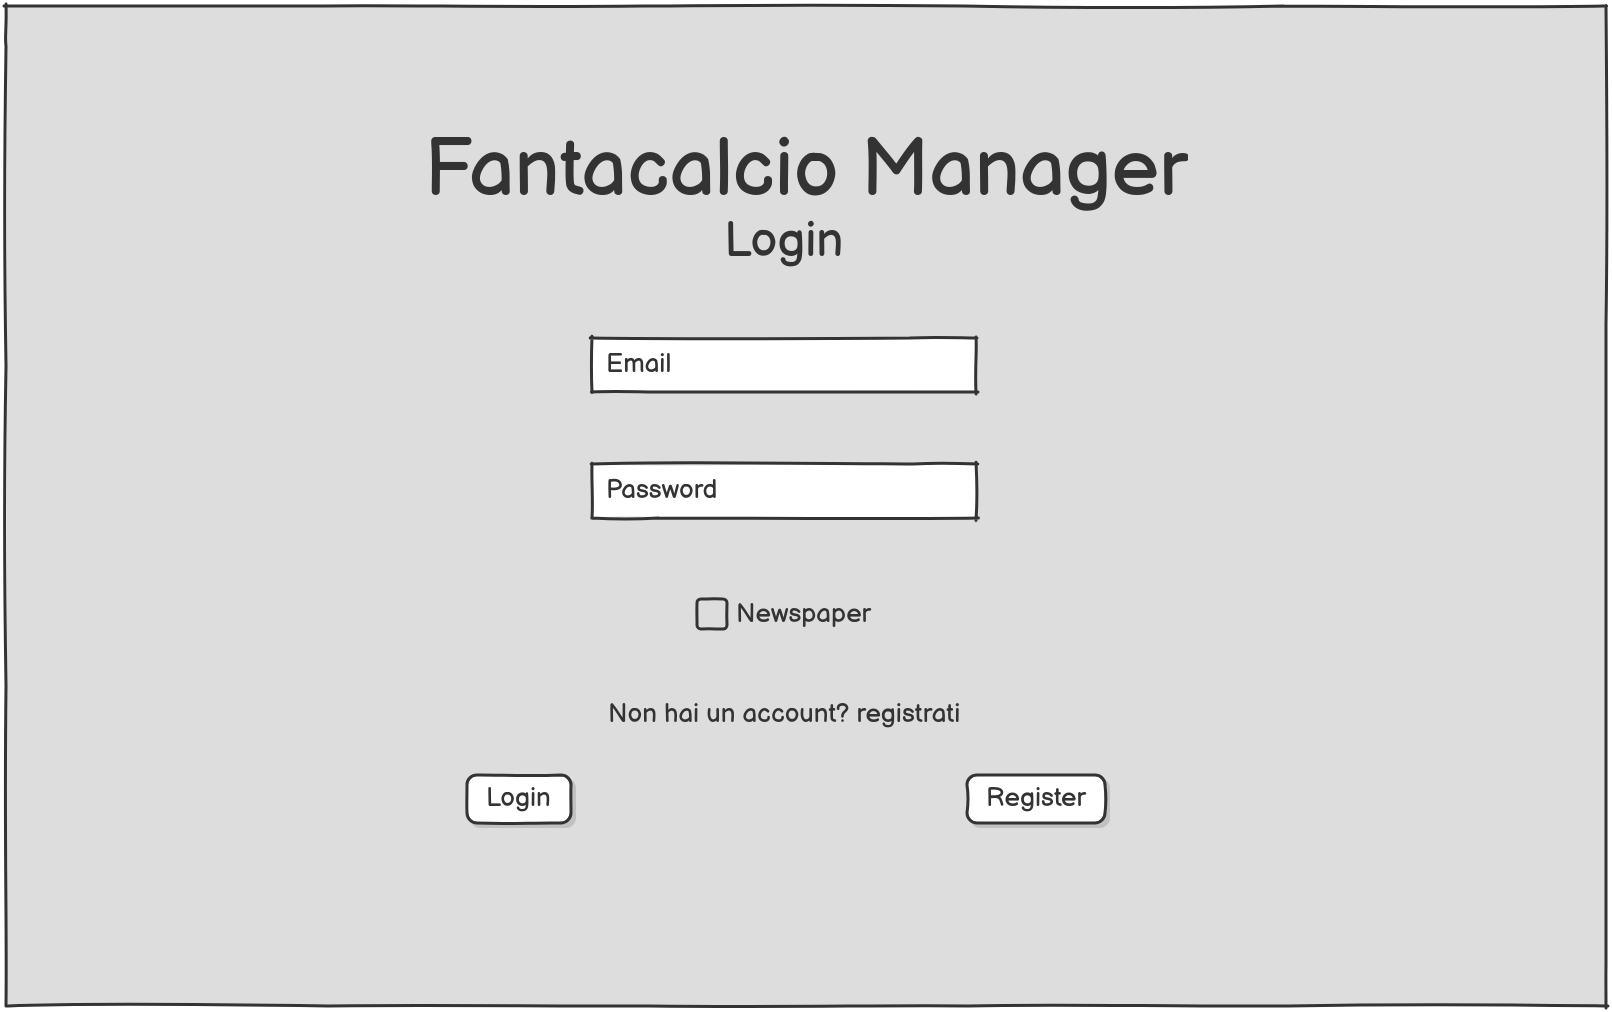
\includegraphics[width=\textwidth]{Resources/Mockups/Login.png}
        \caption{Mockup della pagina di login.}
        \label{fig:pagina_login}
    \end{subfigure}
    \hfill
    \begin{subfigure}[b]{0.49\textwidth}
        \centering
        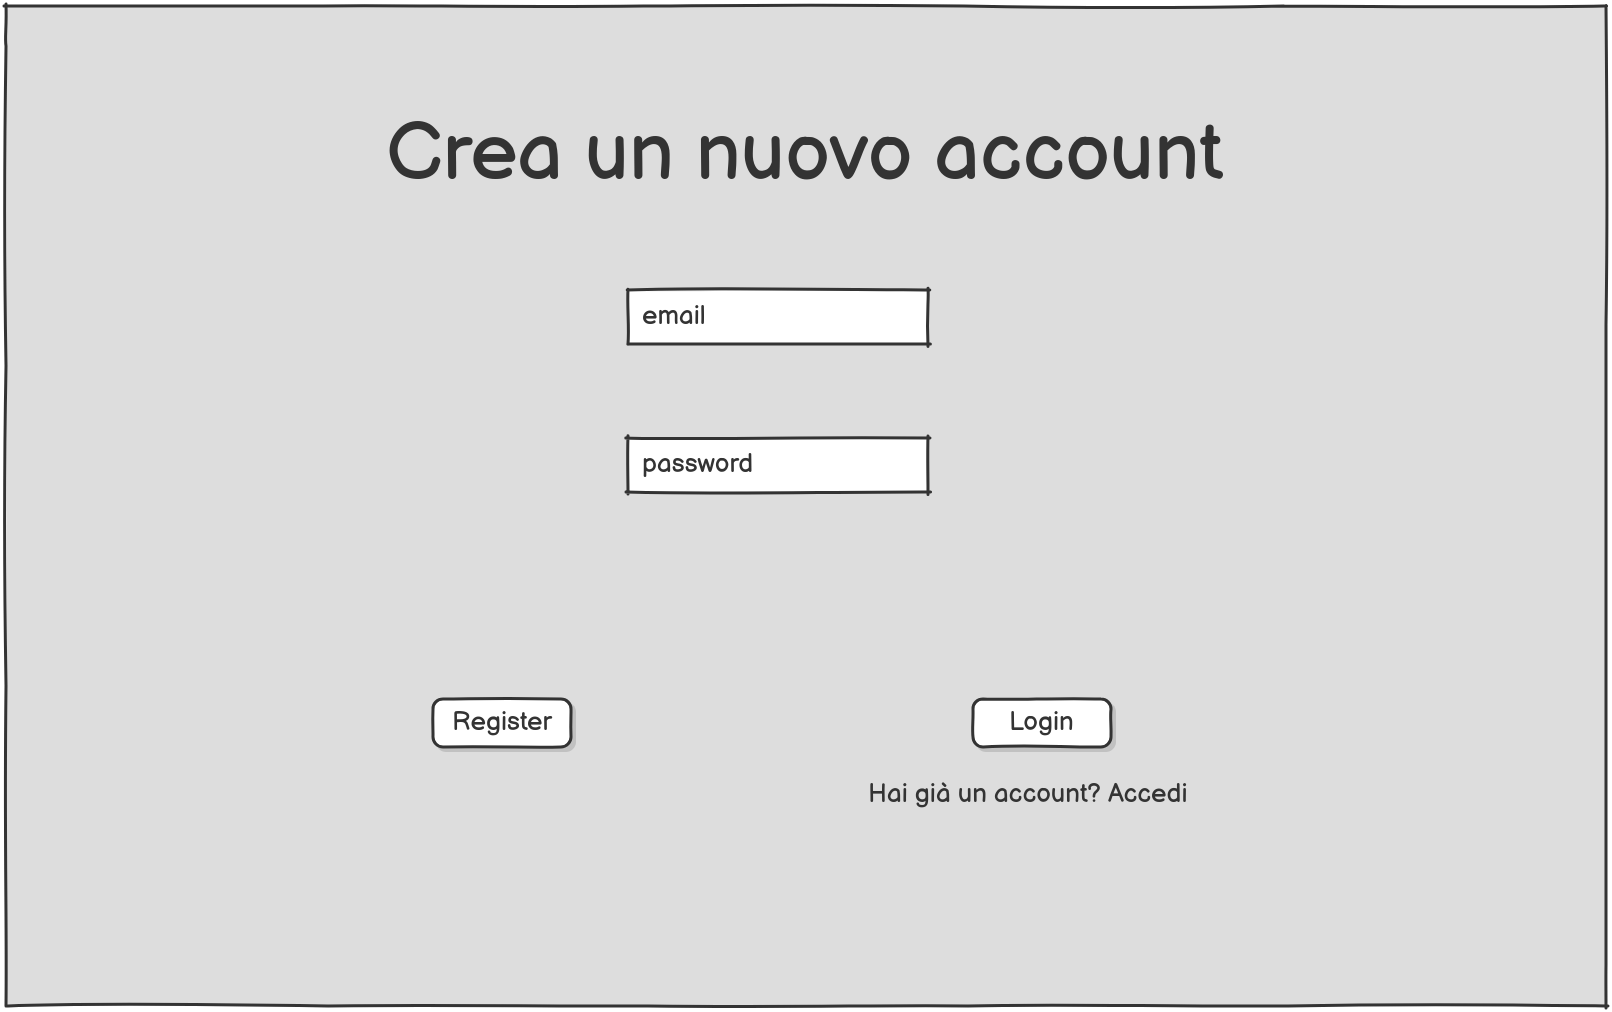
\includegraphics[width=\textwidth]{Resources/Mockups/Registrazione.png}
        \caption{Mockup della pagina di registrazione.}
        \label{fig:pagina_registrazione}
    \end{subfigure}

    % 2ª riga
    \begin{subfigure}[b]{0.49\textwidth}
        \centering
        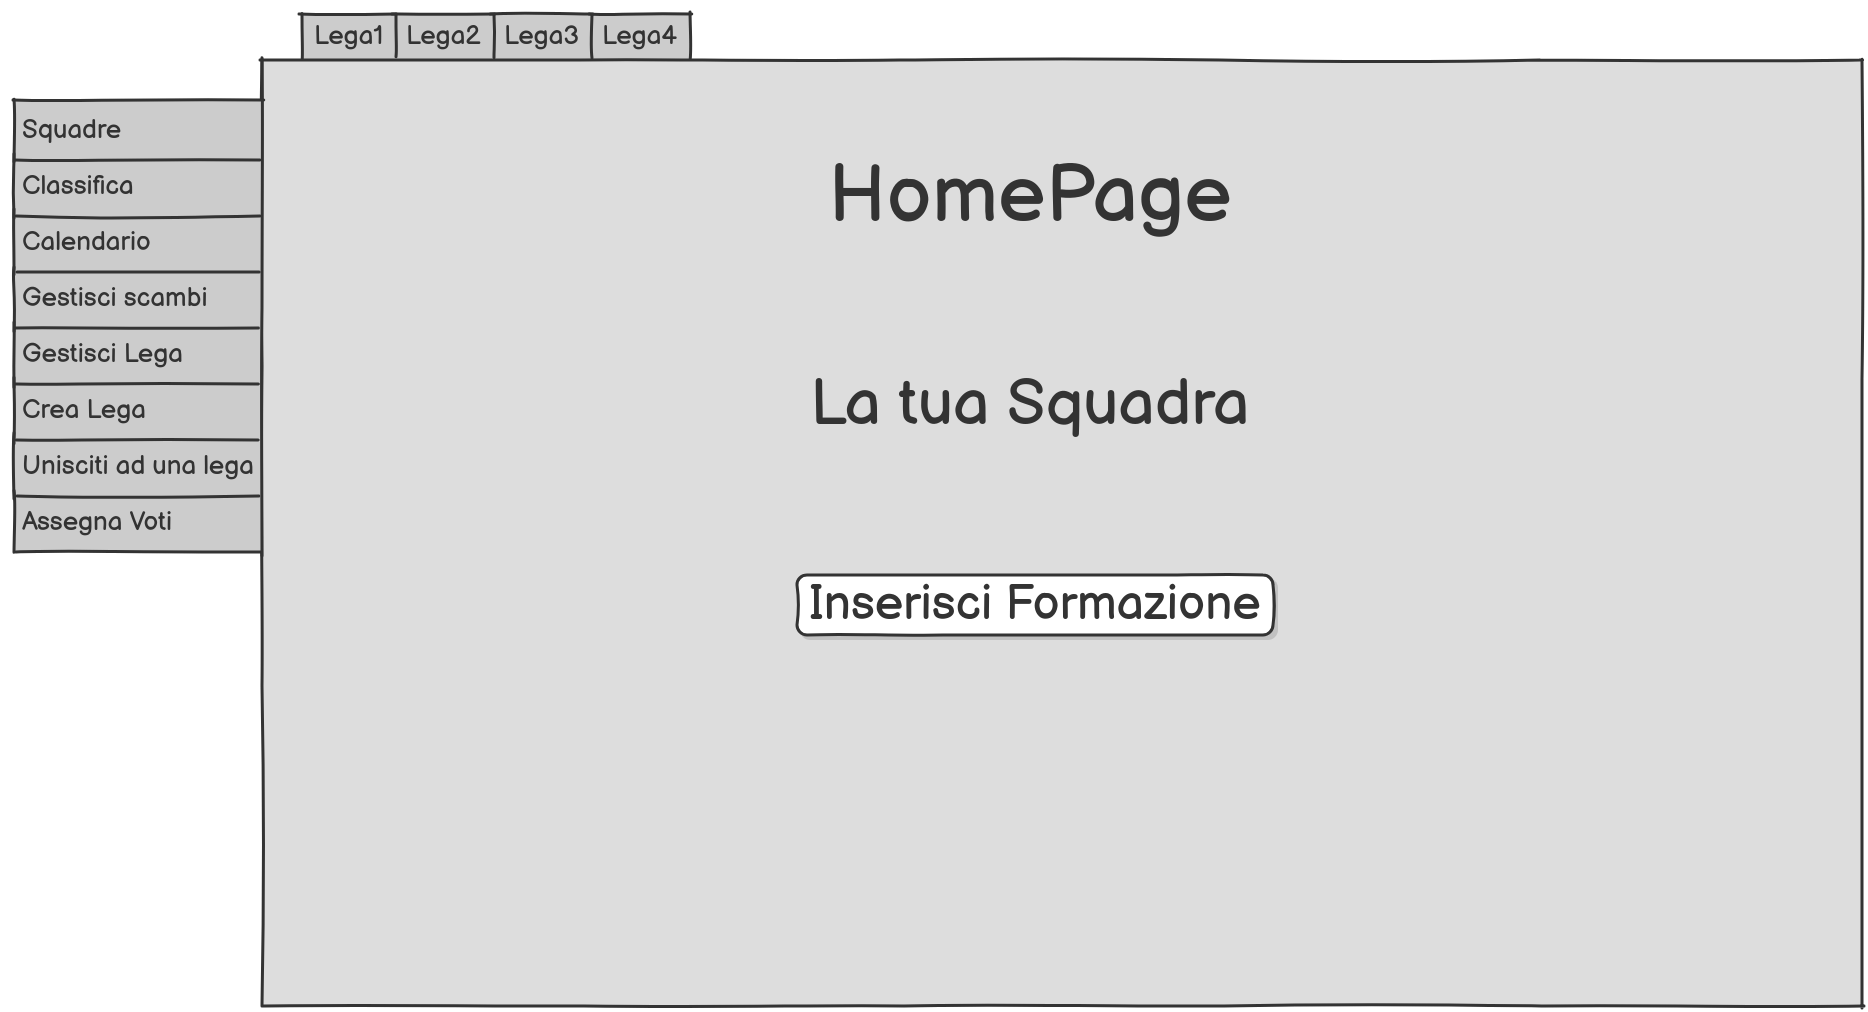
\includegraphics[width=\textwidth]{Resources/Mockups/HomePage.png}
        \caption{Mockup della homepage.}
        \label{fig:pagina_homepage}
    \end{subfigure}
    \hfill
    \begin{subfigure}[b]{0.49\textwidth}
        \centering
        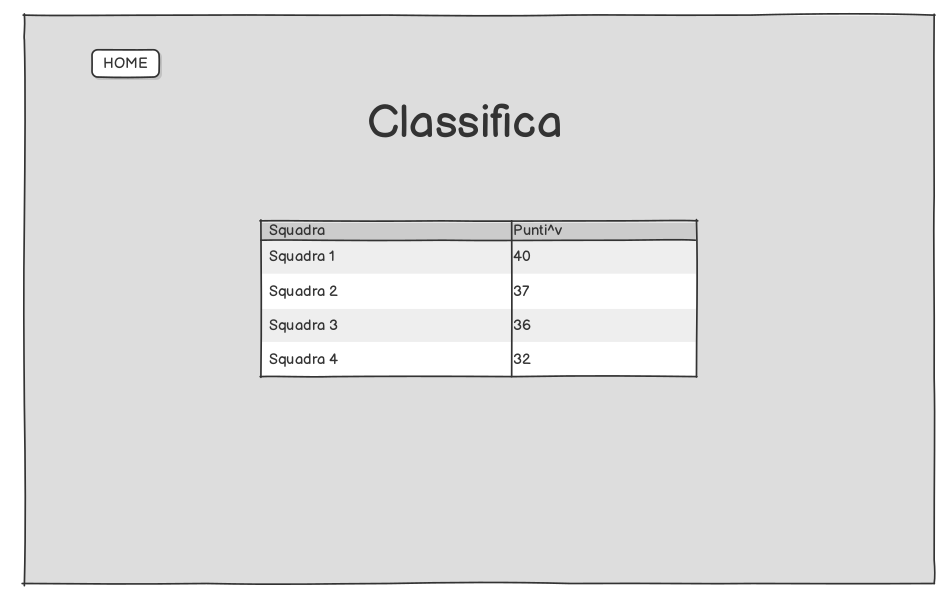
\includegraphics[width=\textwidth]{Resources/Mockups/Classifica.png}
        \caption{Mockup della classifica.}
        \label{fig:pagina_classifica}
    \end{subfigure}

    \caption{Mockup delle pagine di accesso e homepage.}
    \label{fig:mockup_parte1}
\end{figure}
\begin{figure}[H]
    \centering

    % 3ª riga
    \begin{subfigure}[b]{0.49\textwidth}
        \centering
        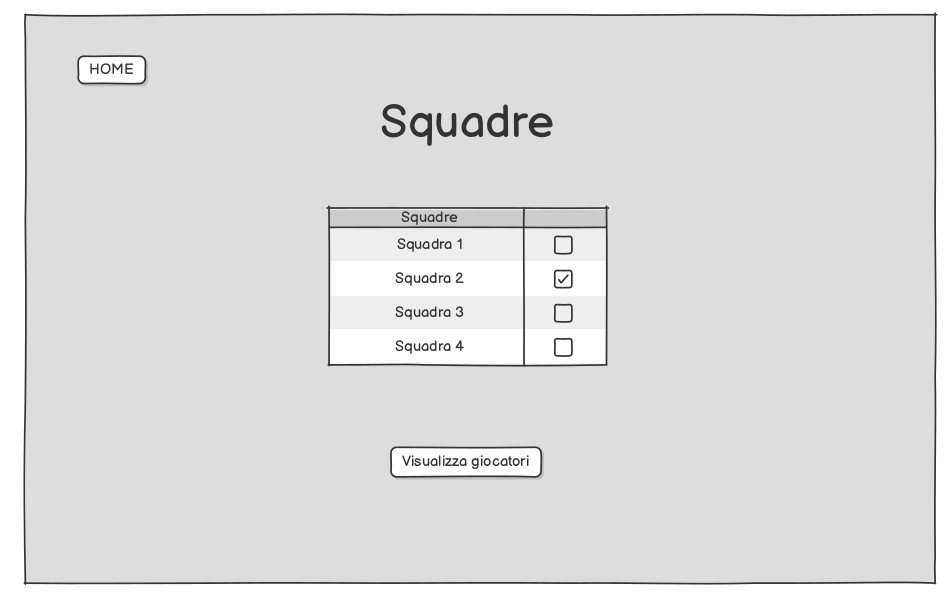
\includegraphics[width=\textwidth]{Resources/Mockups/Squadre.png}
        \caption{Mockup della pagina delle squadre.}
        \label{fig:pagina_squadre}
    \end{subfigure}
    \hfill
    \begin{subfigure}[b]{0.49\textwidth}
        \centering
        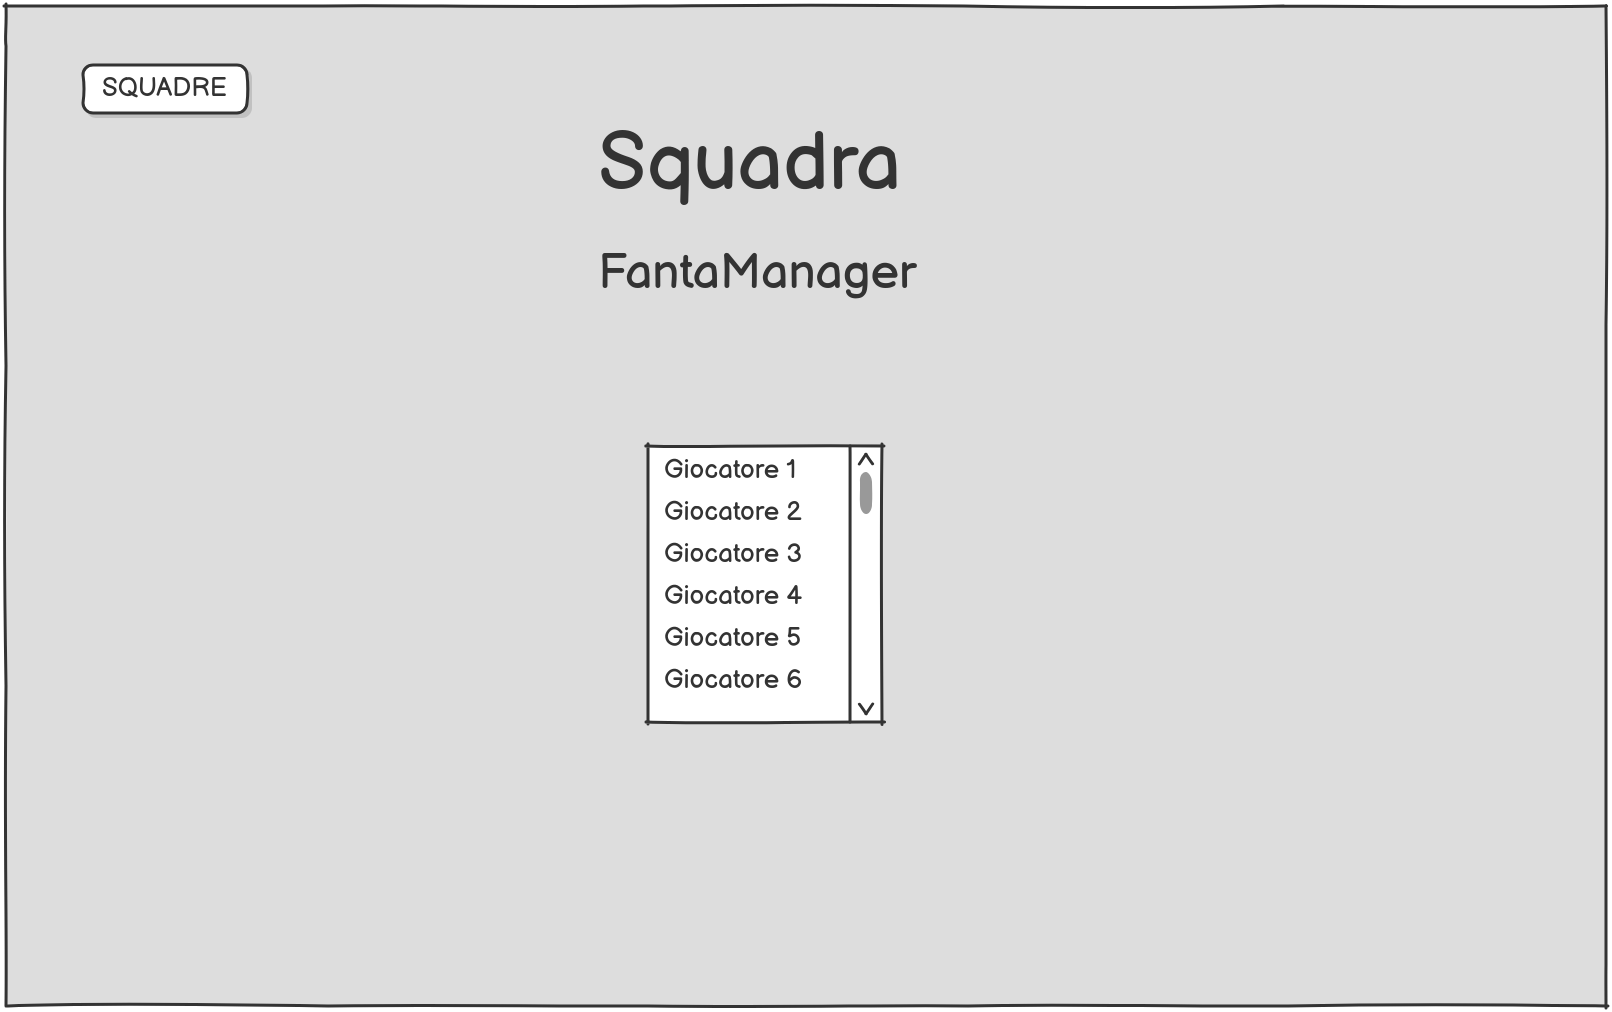
\includegraphics[width=\textwidth]{Resources/Mockups/VisualizzaSquadra.png}
        \caption{Mockup pagina di visualizzazione di un team.}
        \label{fig:pagina_visualizza_squadra}
    \end{subfigure}

    % 4ª riga
    \begin{subfigure}[b]{0.49\textwidth}
        \centering
        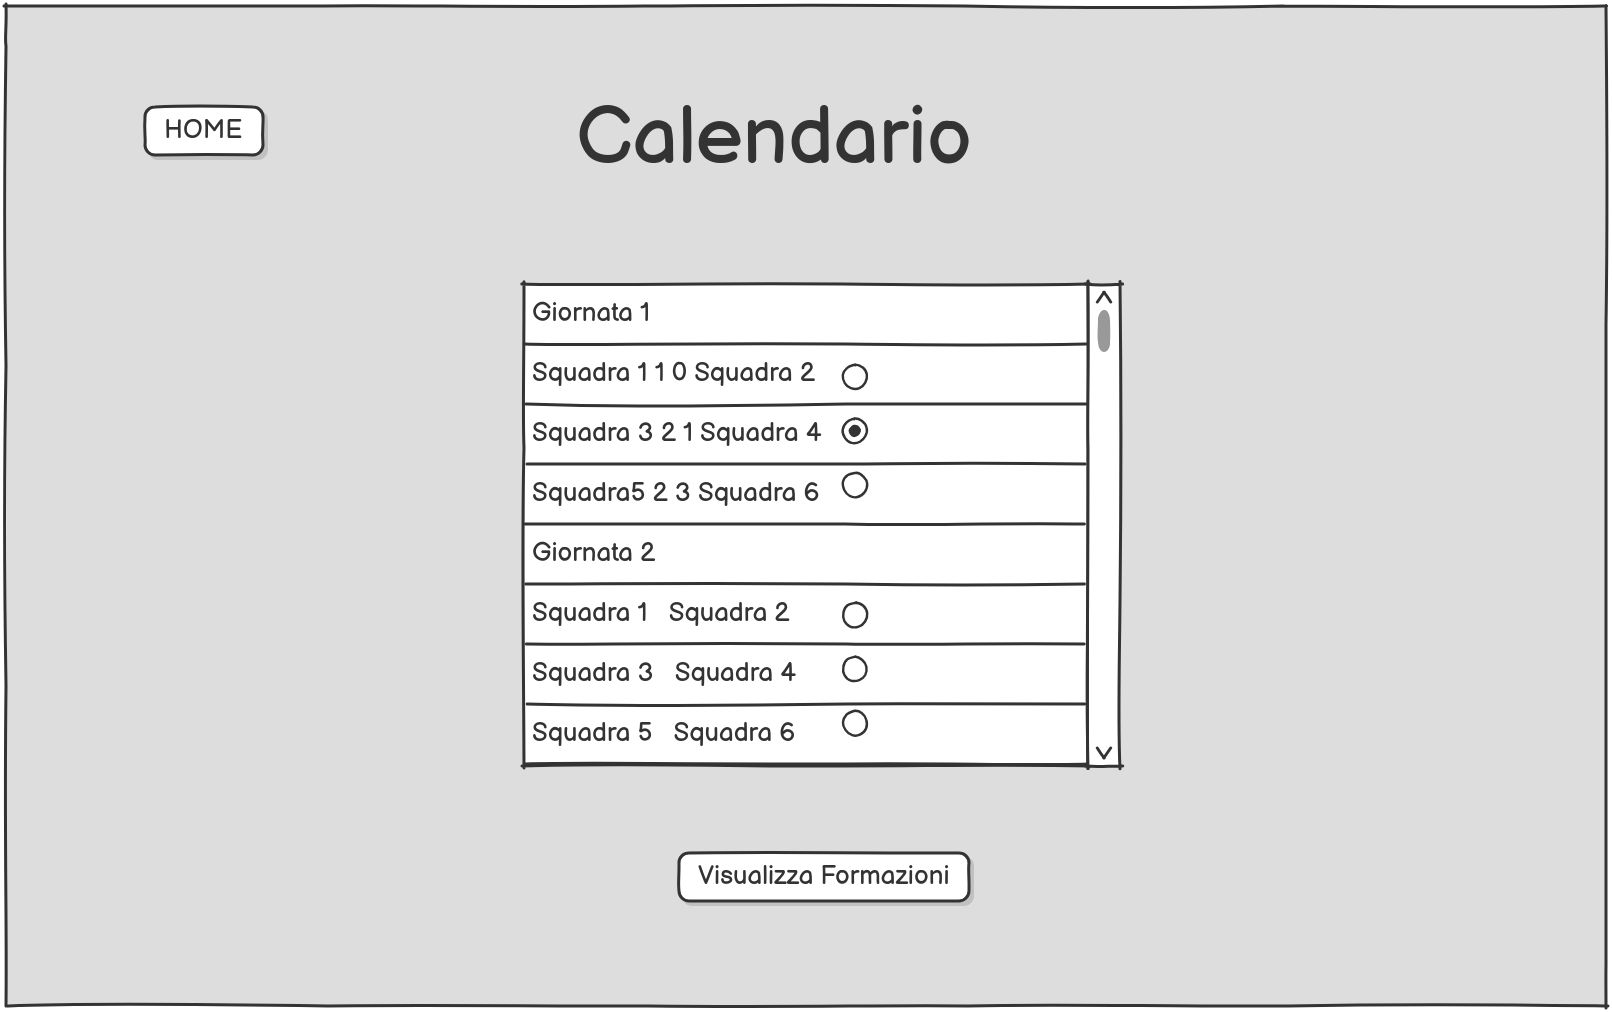
\includegraphics[width=\textwidth]{Resources/Mockups/Calendario.png}
        \caption{Mockup della pagina del calendario.}
        \label{fig:pagina_calendario}
    \end{subfigure}
    \hfill
    \begin{subfigure}[b]{0.49\textwidth}
        \centering
        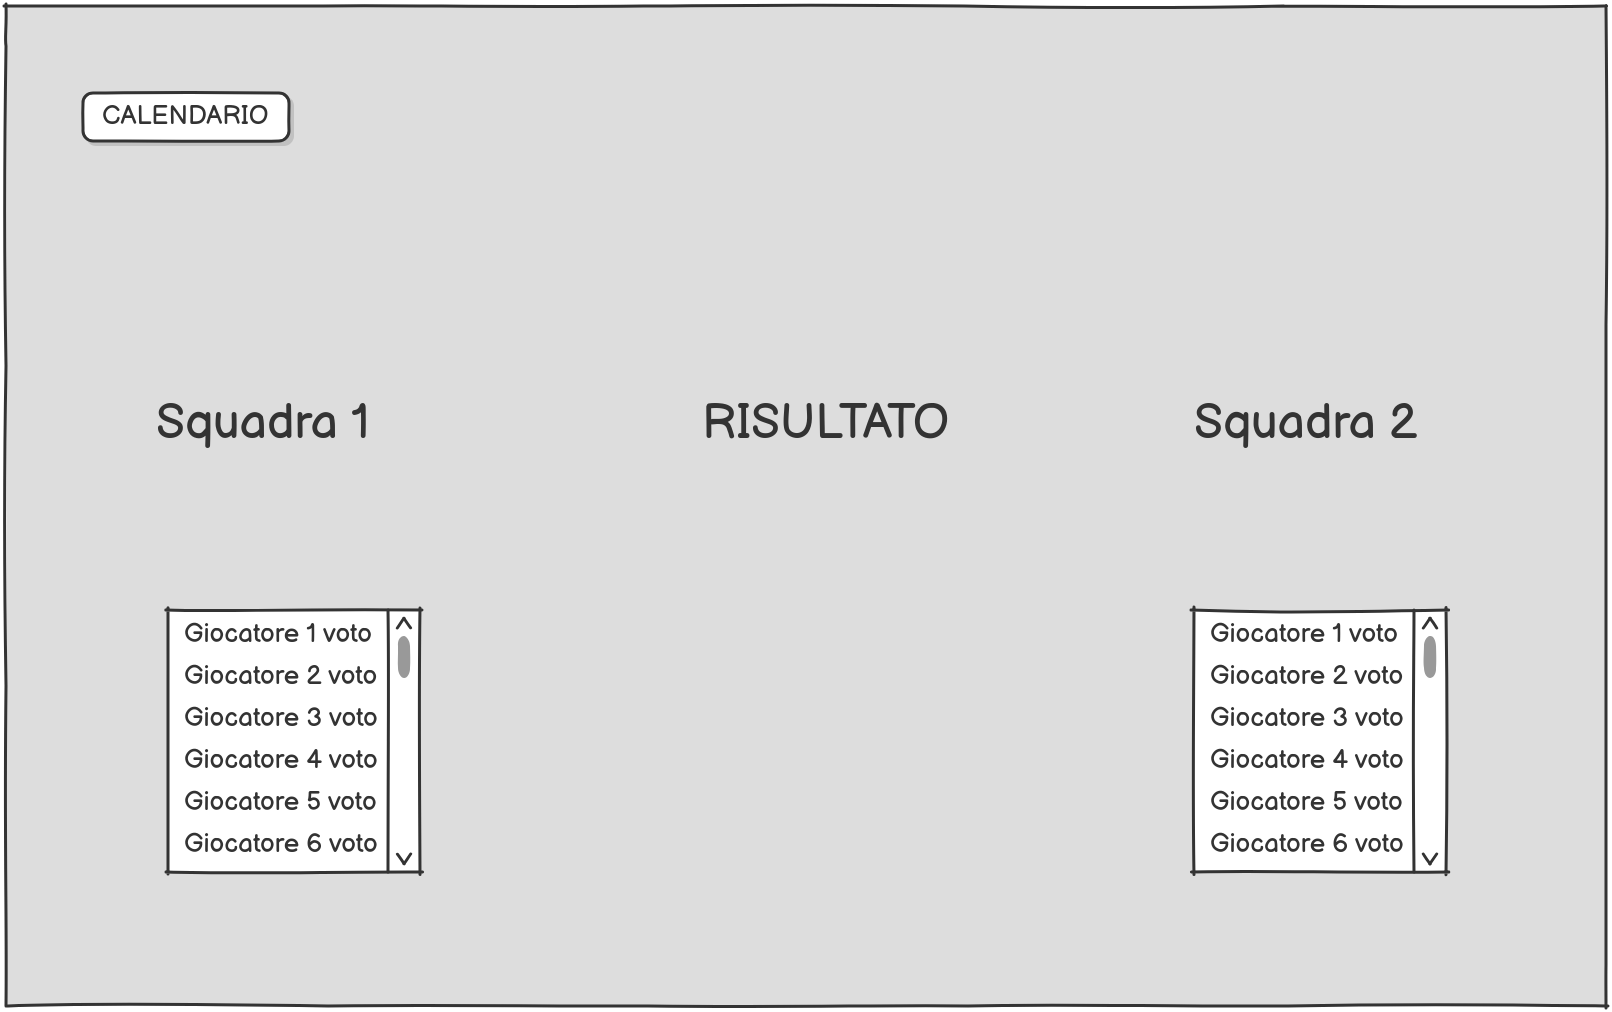
\includegraphics[width=\textwidth]{Resources/Mockups/VisualizzaMatch.png}
        \caption{Mockup pagina di visualizzazione di un match.}
        \label{fig:pagina_visualizza_match}
    \end{subfigure}

    \caption{Mockup delle pagine relative a squadre, calendario e match.}
    \label{fig:mockup_parte2}
\end{figure}
\clearpage
\begin{figure}[H]
    \centering

    % 5ª riga
    \begin{subfigure}[b]{0.49\textwidth}
        \centering
        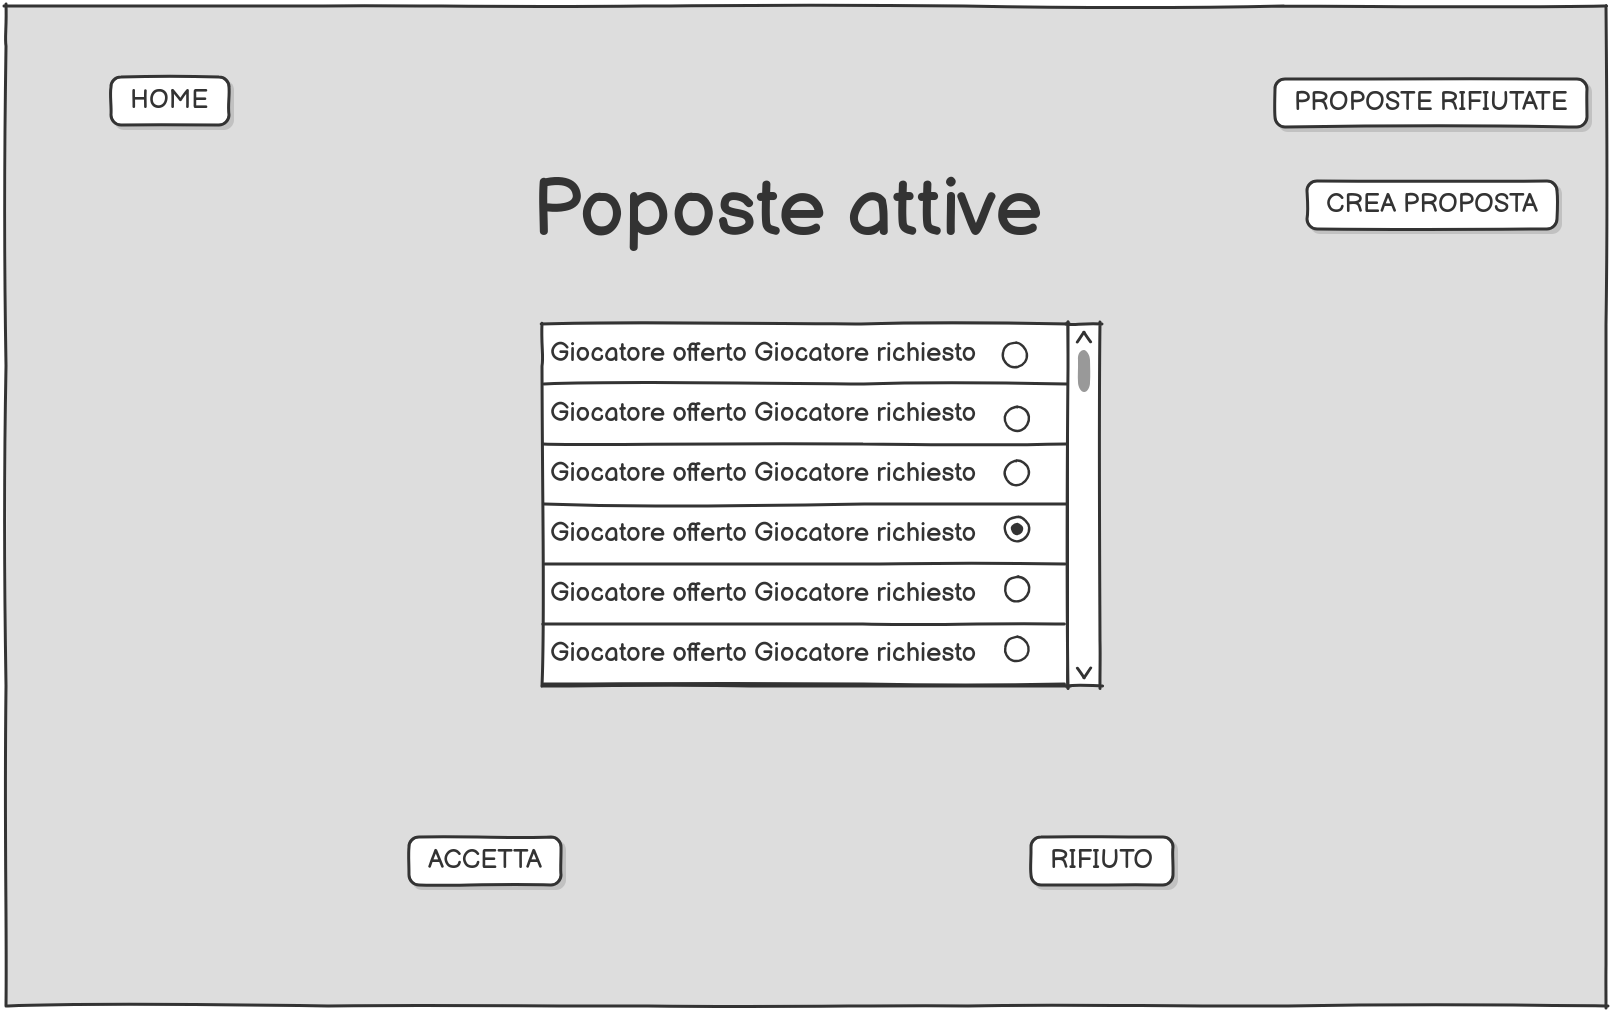
\includegraphics[width=\textwidth]{Resources/Mockups/ProposteAttive.png}
        \caption{Mockup della pagina delle proposte attive.}
        \label{fig:pagina_proposte_attive}
    \end{subfigure}
    \hfill
    \begin{subfigure}[b]{0.49\textwidth}
        \centering
        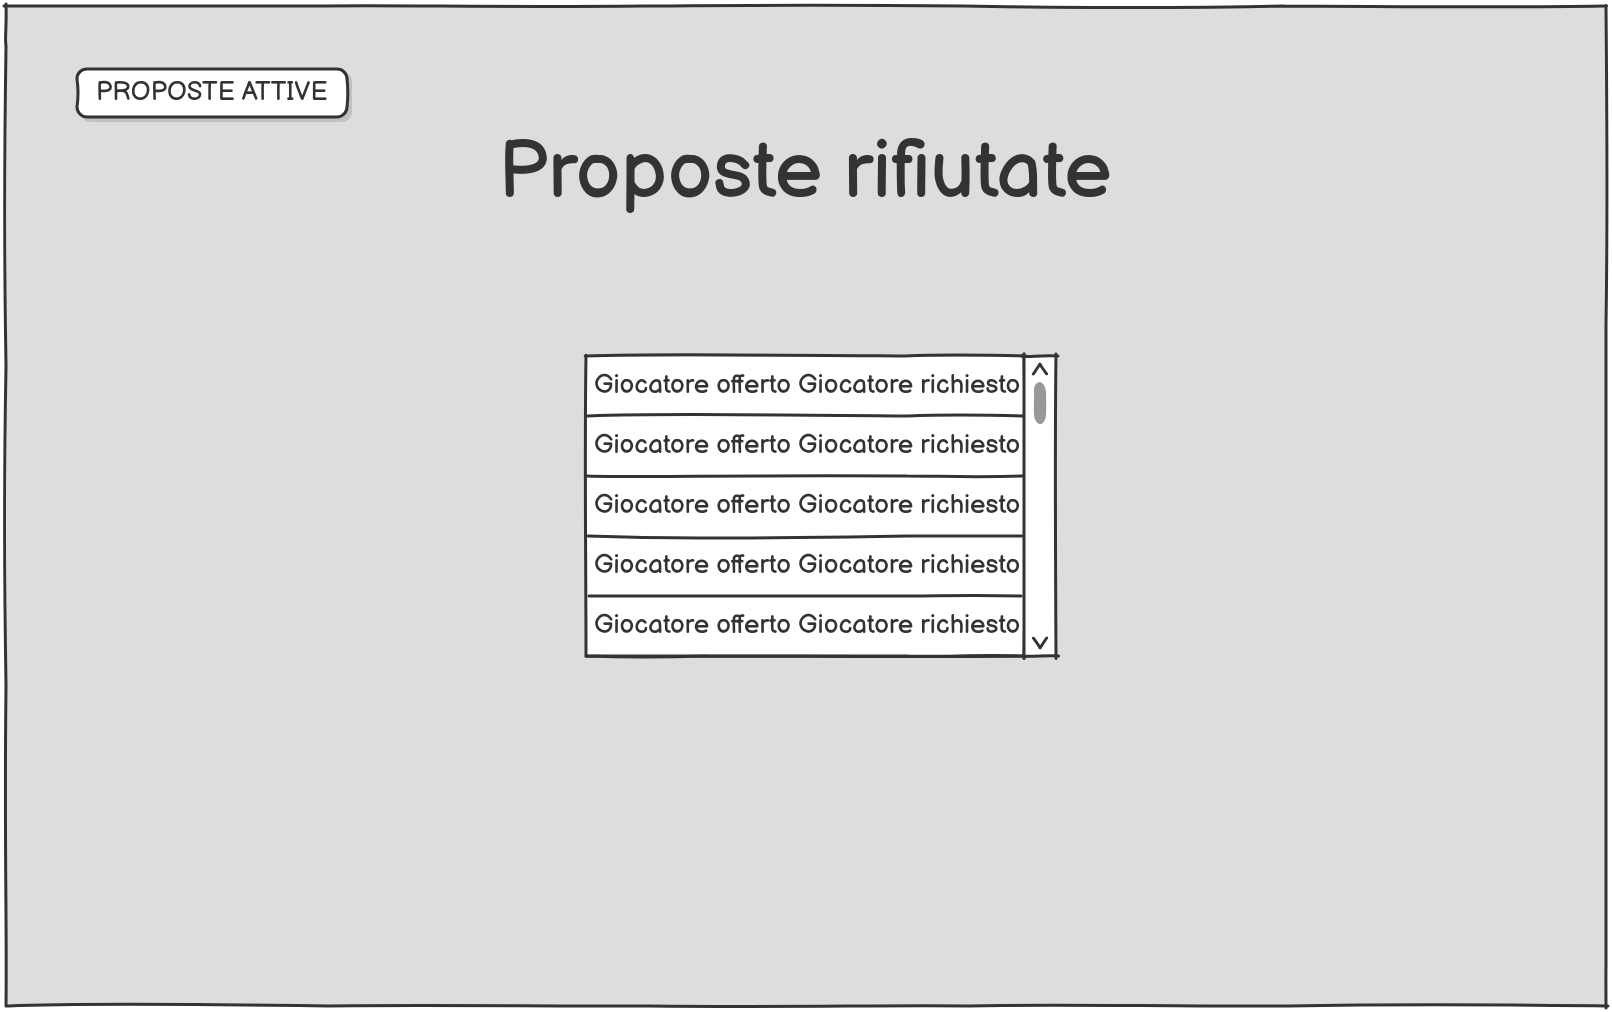
\includegraphics[width=\textwidth]{Resources/Mockups/ProposteRifiutate.png}
        \caption{Mockup della pagina delle proposte rifiutate.}
        \label{fig:pagina_proposte_rifiutate}
    \end{subfigure}

    % 6ª riga
    \begin{subfigure}[b]{0.49\textwidth}
        \centering
        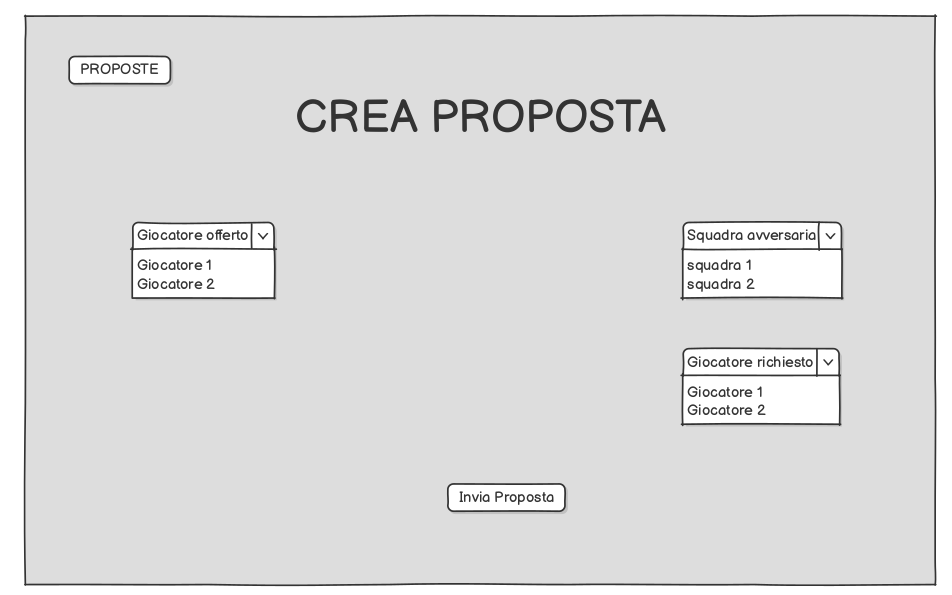
\includegraphics[width=\textwidth]{Resources/Mockups/CreaProposta.png}
        \caption{Mockup pagina per la creazione delle proposte.}
        \label{fig:pagina_crea_proposta}
    \end{subfigure}
    \hfill
    \begin{subfigure}[b]{0.49\textwidth}
        \centering
        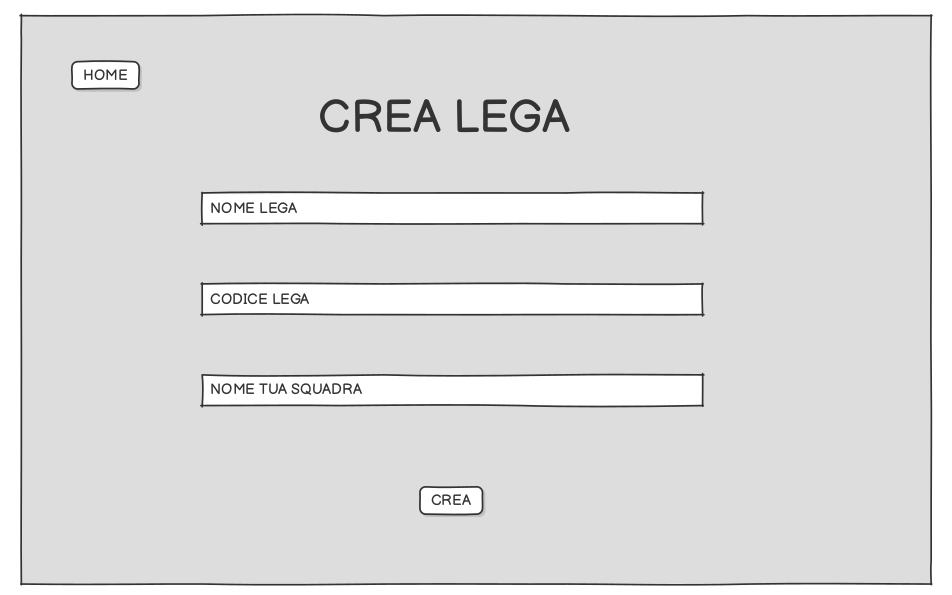
\includegraphics[width=\textwidth]{Resources/Mockups/CreaLega.png}
        \caption{Mockup della pagina di creazione di una lega.}
        \label{fig:pagina_crea_lega}
    \end{subfigure}

    \caption{Mockup delle pagine relative a proposte e creazione di leghe.}
    \label{fig:mockup_parte3}
\end{figure}
\begin{figure}[H]
    \centering

    % 7ª riga
    \begin{subfigure}[b]{0.49\textwidth}
        \centering
        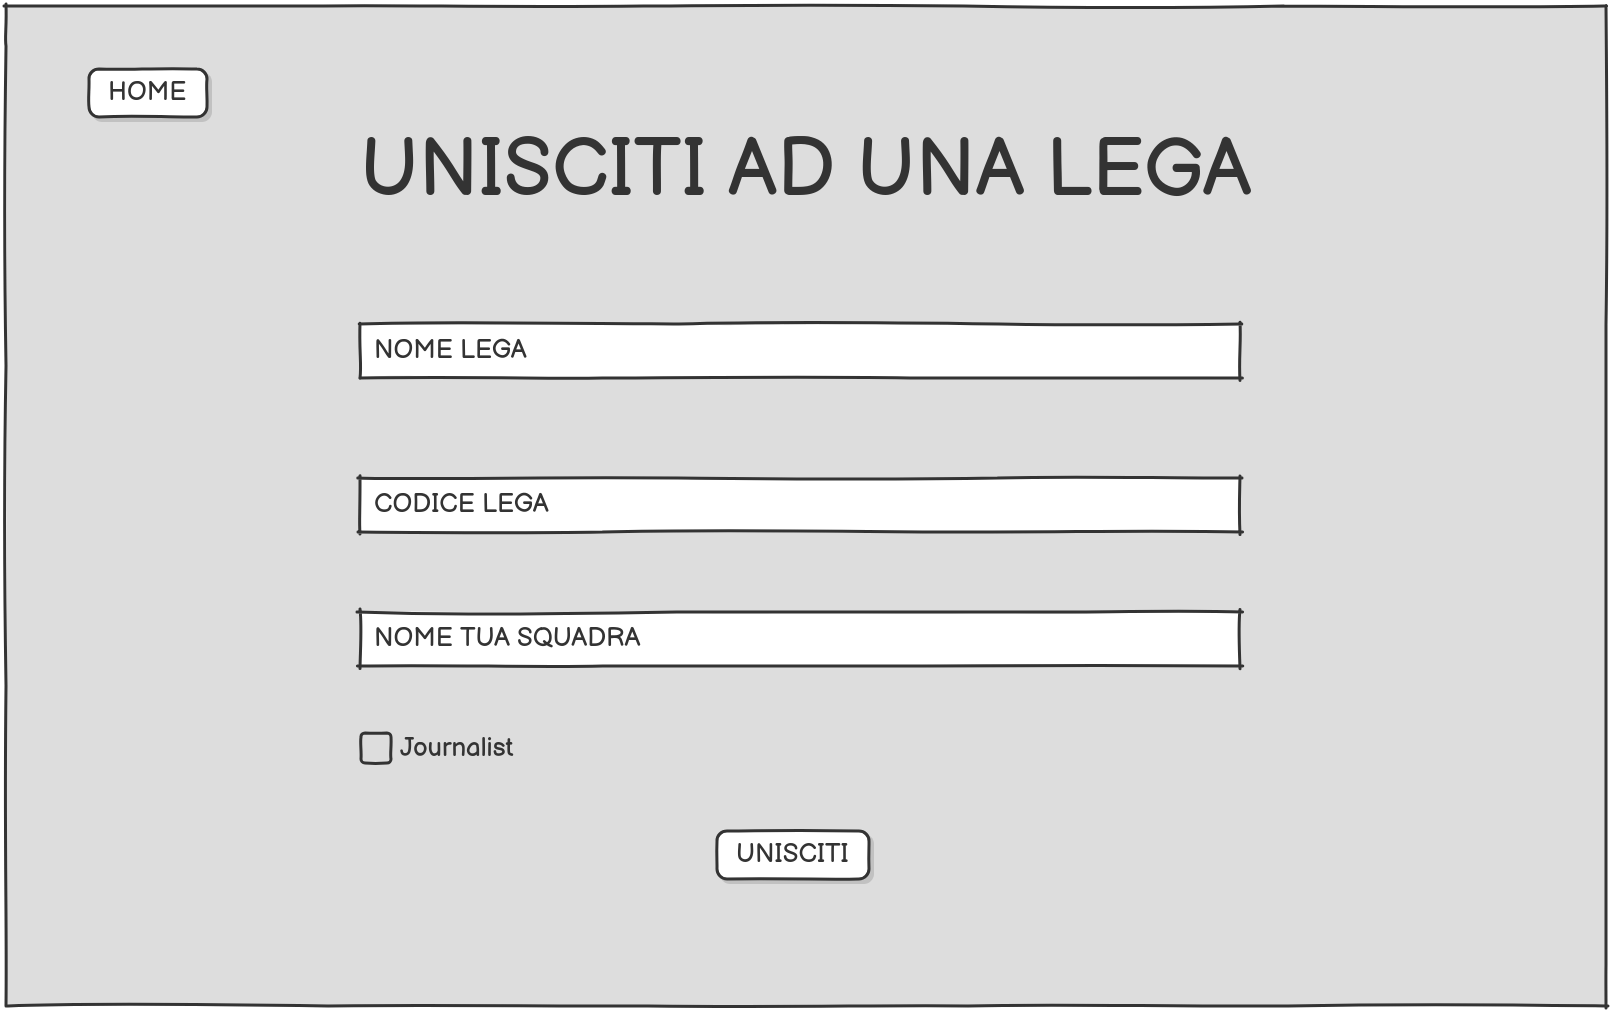
\includegraphics[width=\textwidth]{Resources/Mockups/UniscitiAdUnaLega.png}
        \caption{Mockup della pagina per l'adesione a una lega.}
        \label{fig:pagina_unisciti_lega}
    \end{subfigure}
    \hfill
    \begin{subfigure}[b]{0.49\textwidth}
        \centering
        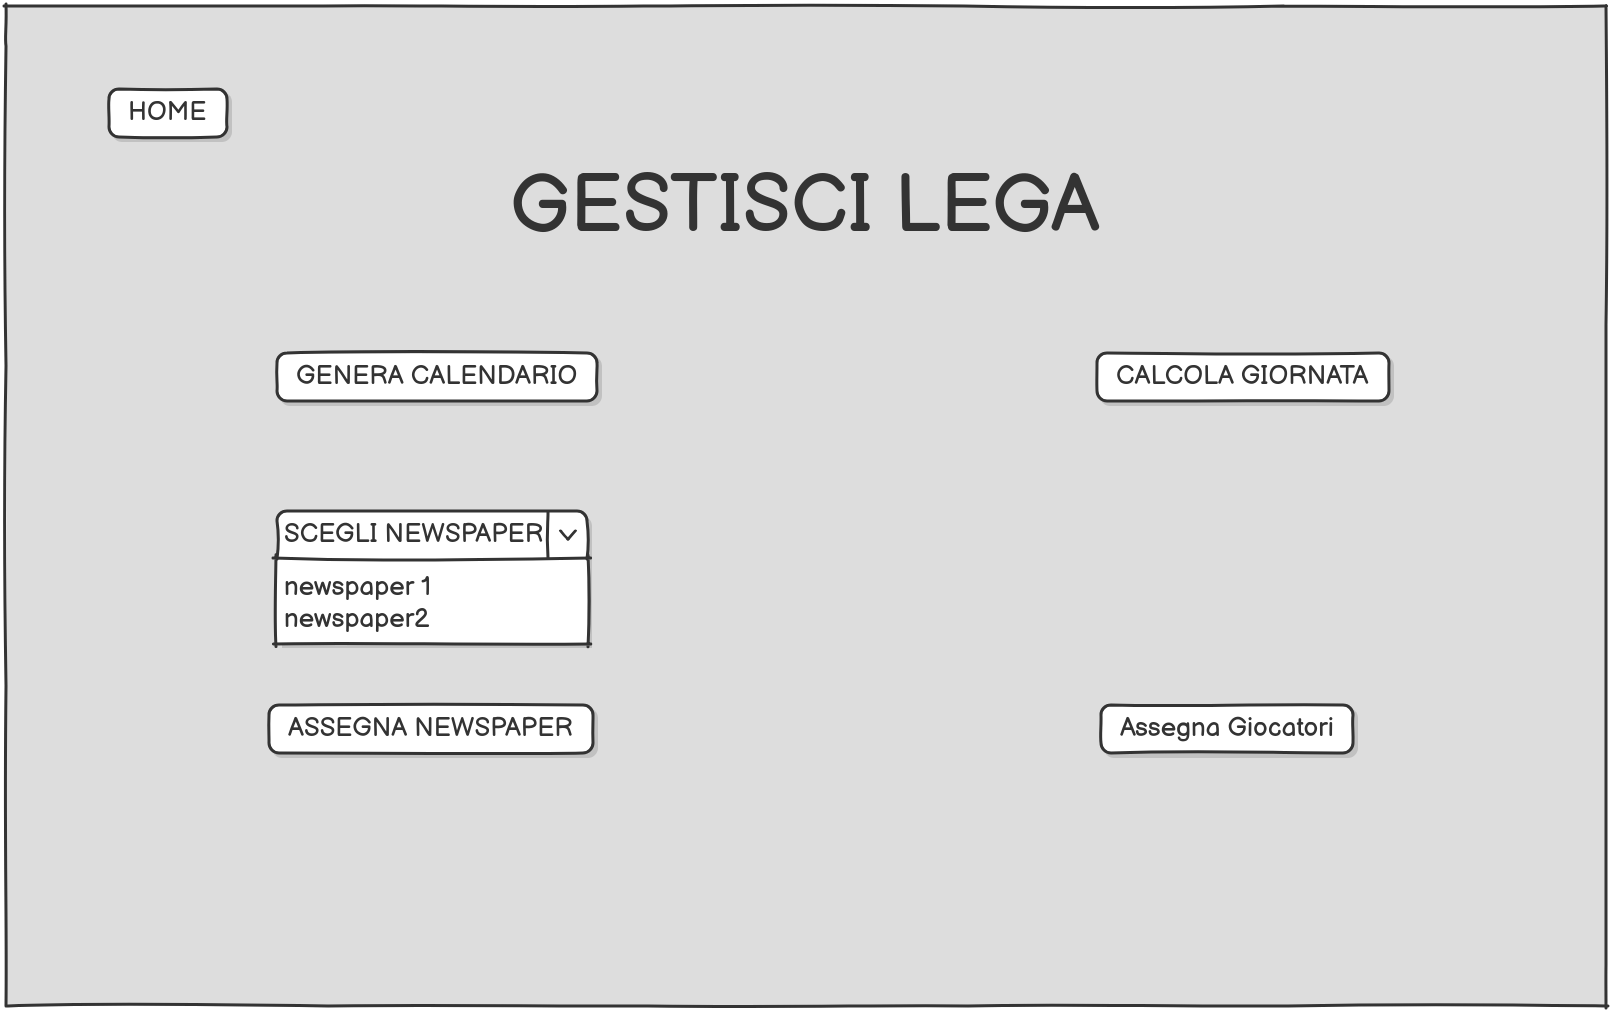
\includegraphics[width=\textwidth]{Resources/Mockups/GestisciLega.png}
        \caption{Mockup della pagina per la gestione della lega.}
        \label{fig:pagina_gestisci_lega}
    \end{subfigure}

    % 8ª riga
    \begin{subfigure}[b]{0.49\textwidth}
        \centering
        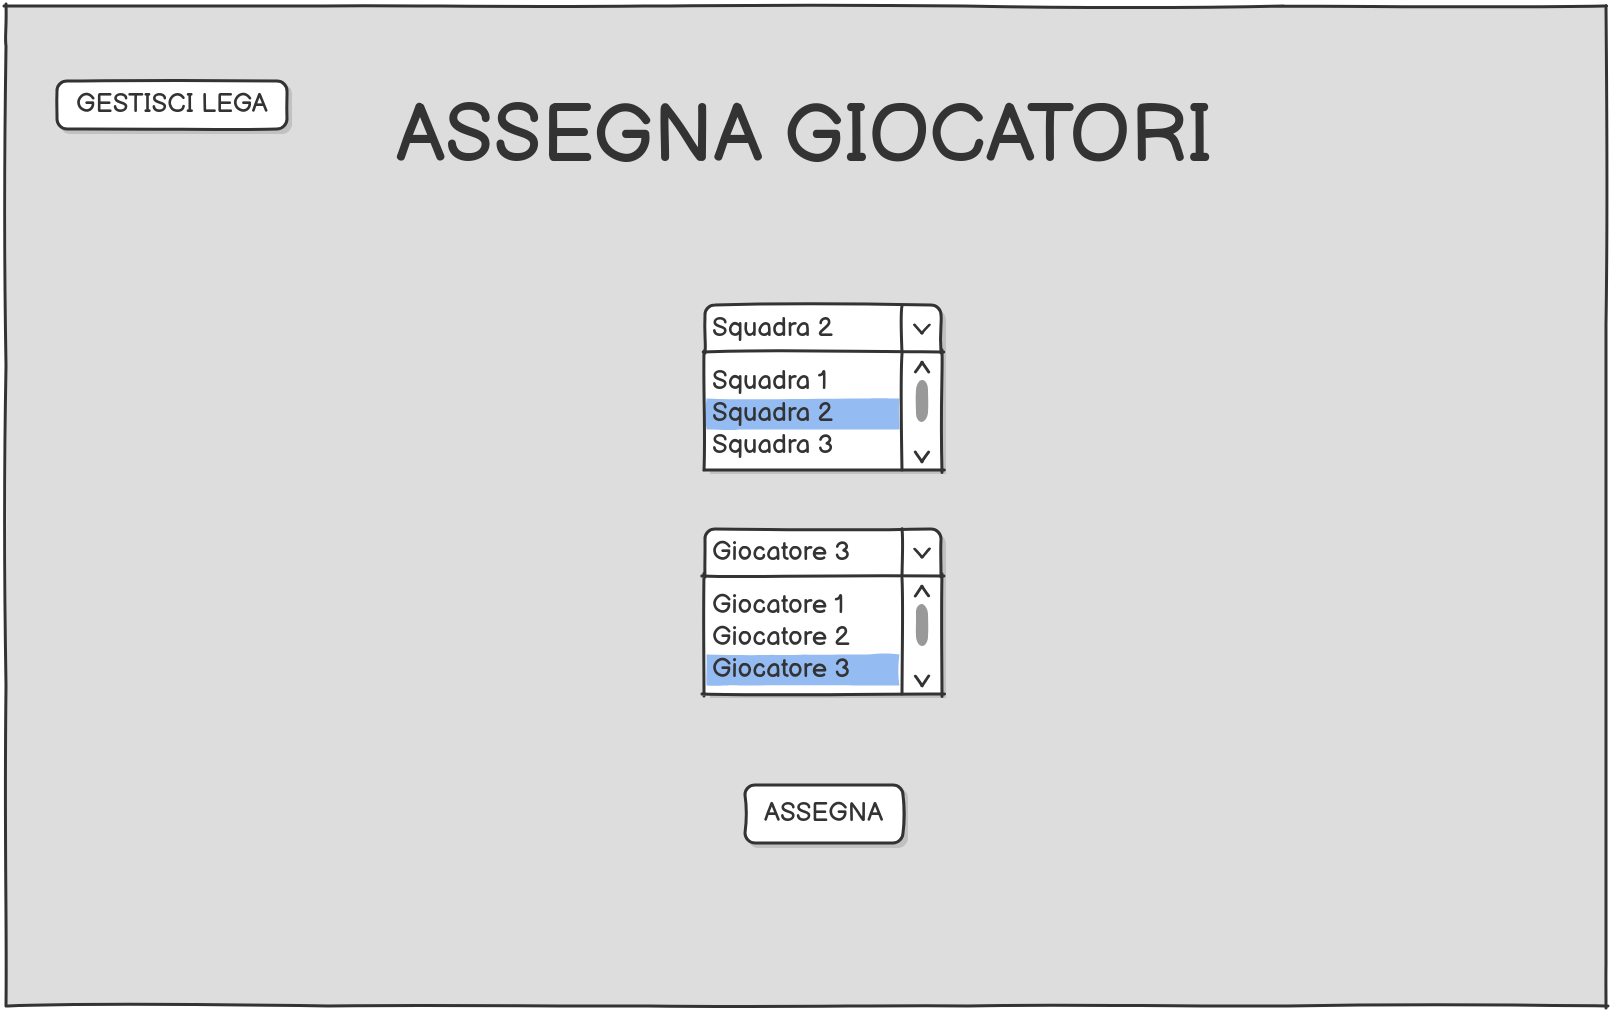
\includegraphics[width=\textwidth]{Resources/Mockups/AssegnaGiocatori.png}
        \caption{Mockup pagina assegnazione dei giocatori ai team.}
        \label{fig:pagina_assegna_giocatori}
    \end{subfigure}
    \hfill
    \begin{subfigure}[b]{0.49\textwidth}
        \centering
        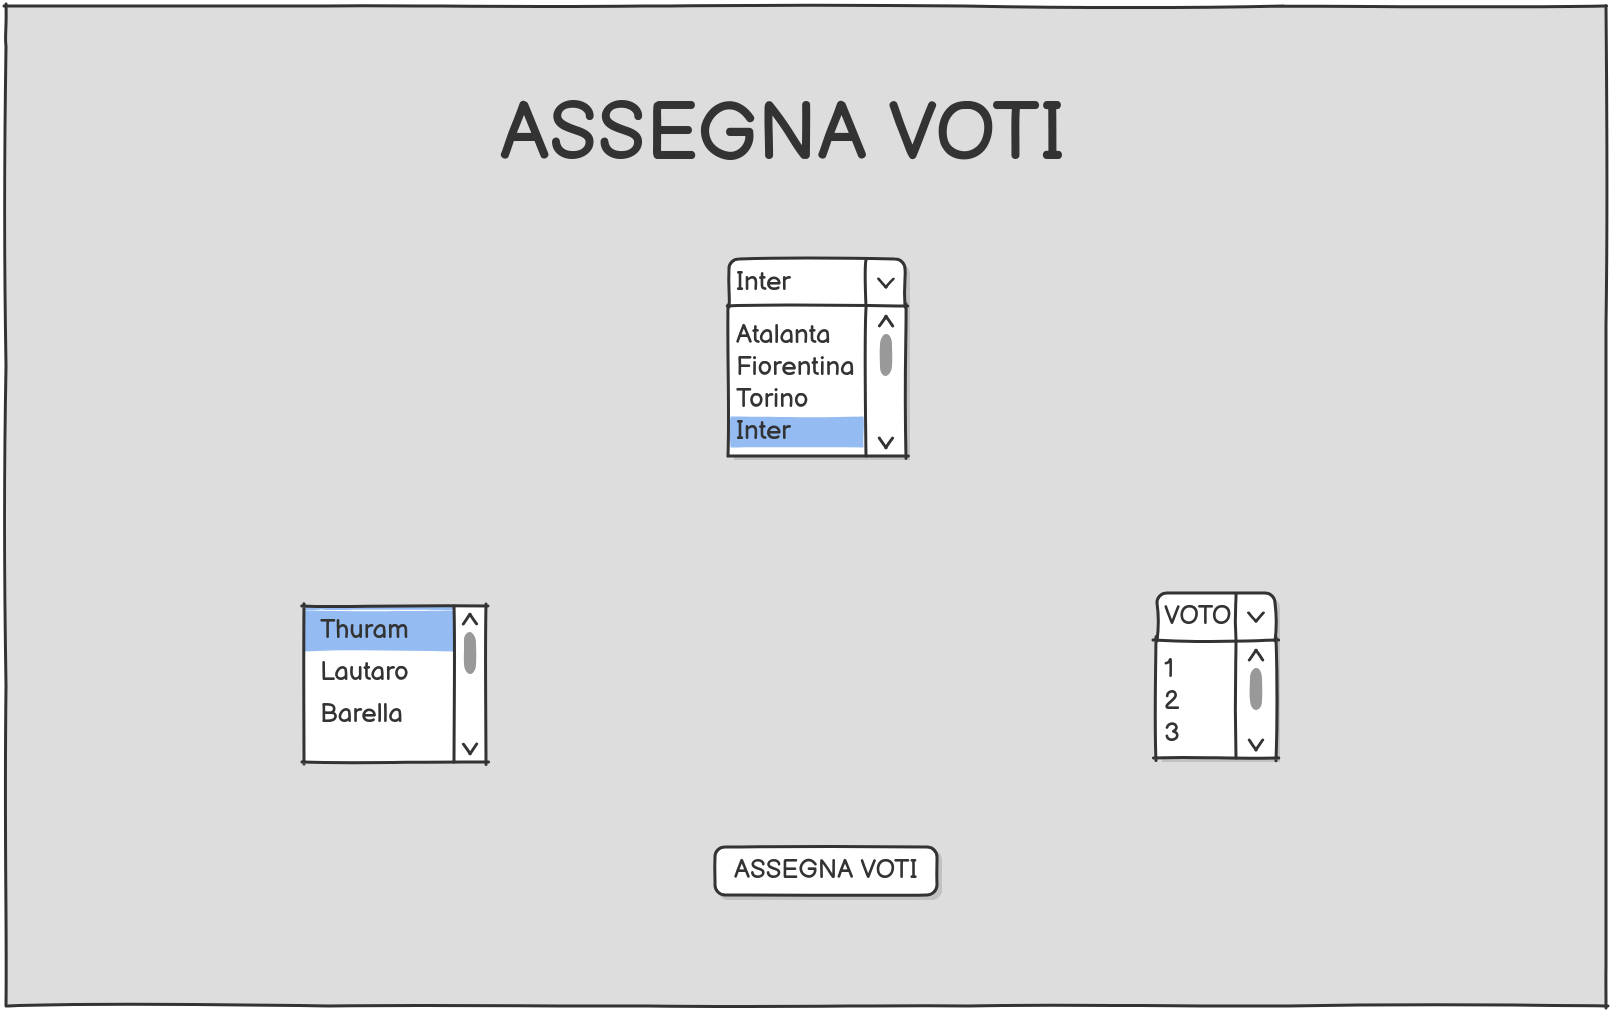
\includegraphics[width=\textwidth]{Resources/Mockups/AssegnaVoti.png}
        \caption{Mockup della pagina per l'assegnazione dei voti.}
        \label{fig:pagina_assegna_voti}
    \end{subfigure}

    \caption{Mockup delle pagine di gestione delle leghe e assegnazioni.}
    \label{fig:mockup_parte4}
\end{figure}


\section{Implementazione}
\todo{Parlare del domain model, delle annotazioni, dei repository, dei service forse è più adatto qui parlare approfonditamente del databse ed in progettazione fare un introduzione}
\todo[color=blue]{Qui parla di come hai implementato il transaction manager, E Gui approfondita}
In questa sezione verrà descritta l'implementazione dell'applicazione analizzandone tutti
i componenti.
\subsection{Domain Model}
\begin{figure}
    \centering
    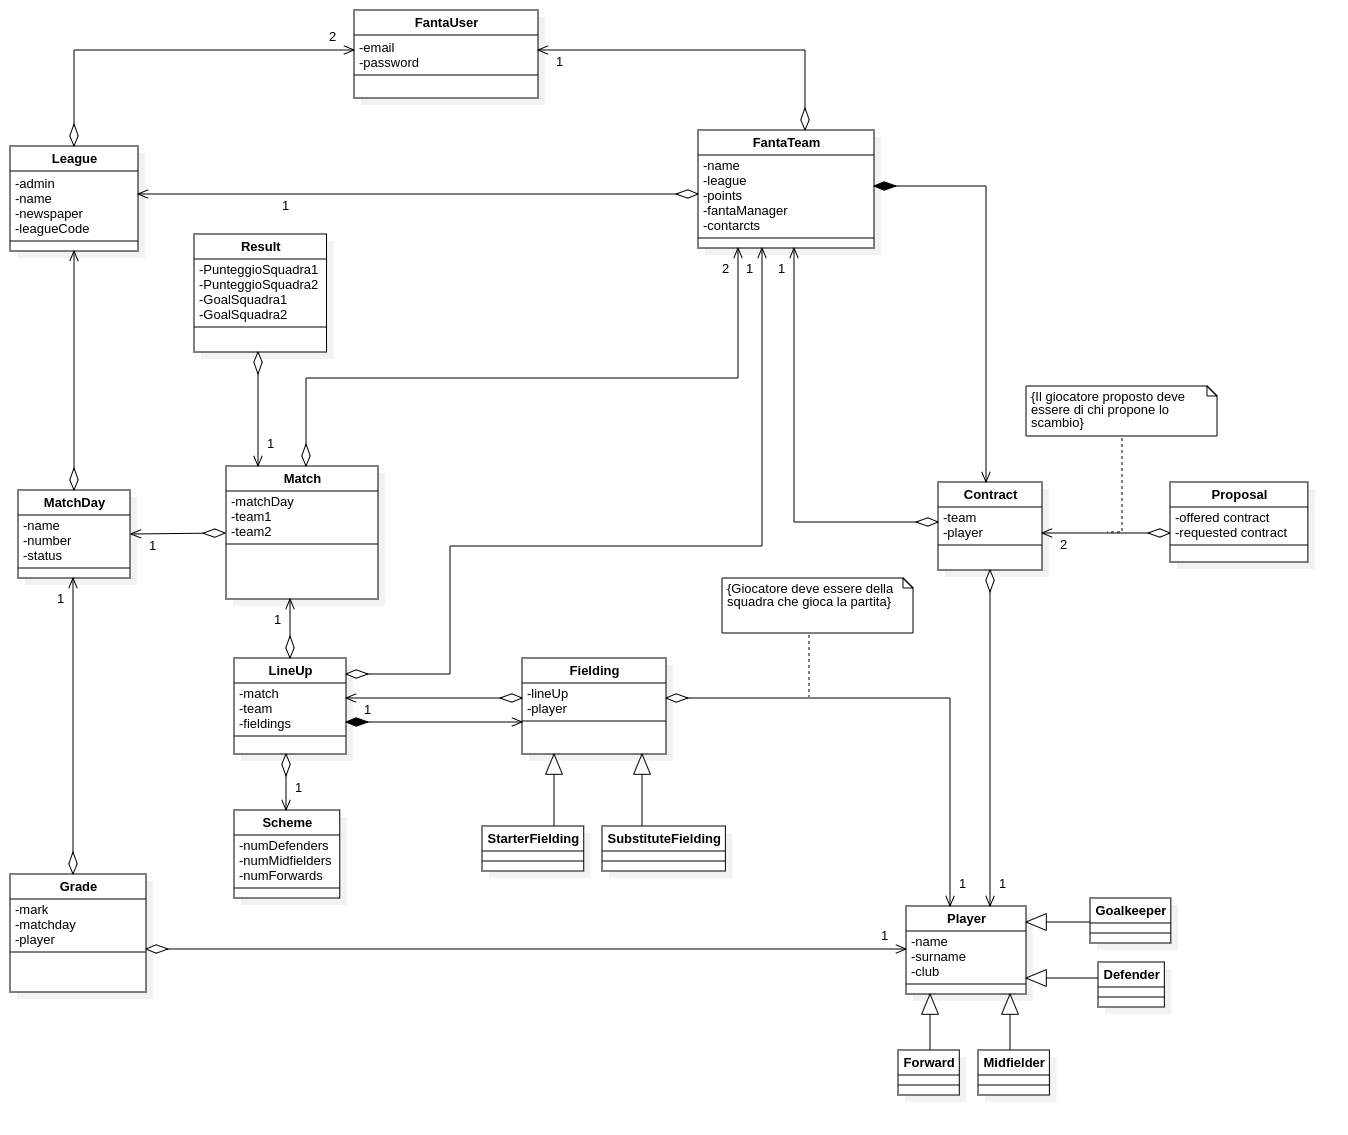
\includegraphics[width=\textwidth]{Resources/graficiUML/ClassDiagram.png}        
    \caption{Domain class diagram.}
    \label{fig:domain_class_diagram2}
\end{figure}
Il domainn model rappresnta le entità di dominio del sistema e le loro relazioni.
Tutte le classi presenti sono state annotate con \textbf{Jpa}.
La classe \textbf{League} rappresenta la lega. Essa ha un nome, un codice ed un riferimento
a due user l'admin e il journalist. La classe \textbf{fantaUser} rappresenta l'utente che può
svolgere varie azioni in base al ruolo che ricopre nella lega. La classe \textbf{FantaTeam}
rappresenta il team di un utente all'interno di una lega. È interessante riportare
che la classe \textbf{FantaTeam} ha una relazione bidirezionale con la classe \textbf{Contract},
ciò è sato implementato con la relazione \textbf{Jpa MappedBy}, nella sezione su \textbf{Jpa}
verranno approfonditi i motivi di questa scelta.Inoltre è presente la classe \textbf{FantateamViewer}
che non è nient'altro che un visitor per estrarre il calciatori di un team in base al ruolo. La classe \textbf{Contract} rappresenta l'assegnazione di un
calciatore ad un determinato team. La classe \textbf{Proposal} rappresenta la proposta di scambio
di due calciatori appartenenti a due team della stessa lega. La classe \textbf{Player} rappresenta il calciatore. Il
campo \textit{club} del calciatore rappresenta la squadra reale ed è realizzata con un enum.
Per distinguere tra i vari ruoli di un calciatore abbiamo deciso di creare delle sottoclassi per ognuno di essi,
in questo modo si possono aggiungere ulteriori ruoli per rendere più realistico il gioco.
Per rappresentare le giornate da giocare di una specifica lega è presente la classe \textbf{Matchday}. Ogni giornata è numerata
ed ha uno status rappresentato tramite un enum, in questo modo è possibile stabilire lo stato di avanzamento del gioco
per quella determinata lega. Ad ogni match day sono associati i voti dei calciatori
assegnati dal giornalista, la classe che rappresenta ciò è \textbf{Grade}.
In ogni giornata sono presenti più match ognuno dei quali è rappresentato 
dalla classe \textbf{Match}. Ogni match ha il riferimento ai due team coinvolti
ed una volta concluso ha un riferimento alla classe \textbf{Result}, ovvero il suo risultato.
La classe \textbf{LineUp} rappresenta la formazione schierata da un team per un match.
La classe \textbf{Scheme}, che rappresenta il modulo, è utilizzata per fare type mapping di \textbf{LineUp}, ciò
verrà approfondito in seguito. Anche per \textbf{LineUp} è presente una relazione mapppata
con \textbf{Jpa MappedBy} ed è quella con \textbf{Fielding}, che rappresenta lo schiaremento di un giocatore.
Infine è presente una classe \textbf{LineUpViewer} che implementa un'api sequenziabilizzabile e sicura
per instanziare una \textbf{LineUp}.

\subsection{Services}
Nel pacchetto \textit{Business} sono presenti i services, uno per ogni tipo di attore ed uno per il login.
I services utilizzano il \textbf{TransactionManager} per gestire le transazioni con il database.
In particolare vengono utilizzati i due metodi \textit{inTransaction} e \textit{fromTransaction}, il primo esegue la funzione
 passata all'interno di una transazione e non restituisce nulla mentre il secondo restituisce
 il valore della funzione passata. Inoltre attraverso il \textbf{TransactionContext} i services
 sono in grado di utilizzare i repository per effettuare le loro operazioni.
 I services presenti sono:
 \begin{itemize}
    \item \textbf{LoginService}: si occupa di effettuare le operazioni di login e registrazione.
    \item \textbf{UserService}: si occupa di gestire le operazioni di un utente base all'interno di una lega in cui partecipa.
    \item \textbf{AdminUserService}: si occupa gi gestire le operazioni esclusive di un admin all'interno di una lega.
    \item \textbf{NewsPaperService}: si occupa di gestire le operazioni di un giornalista all'interno di una lega.
 \end{itemize}

\begin{figure}
    \centering
    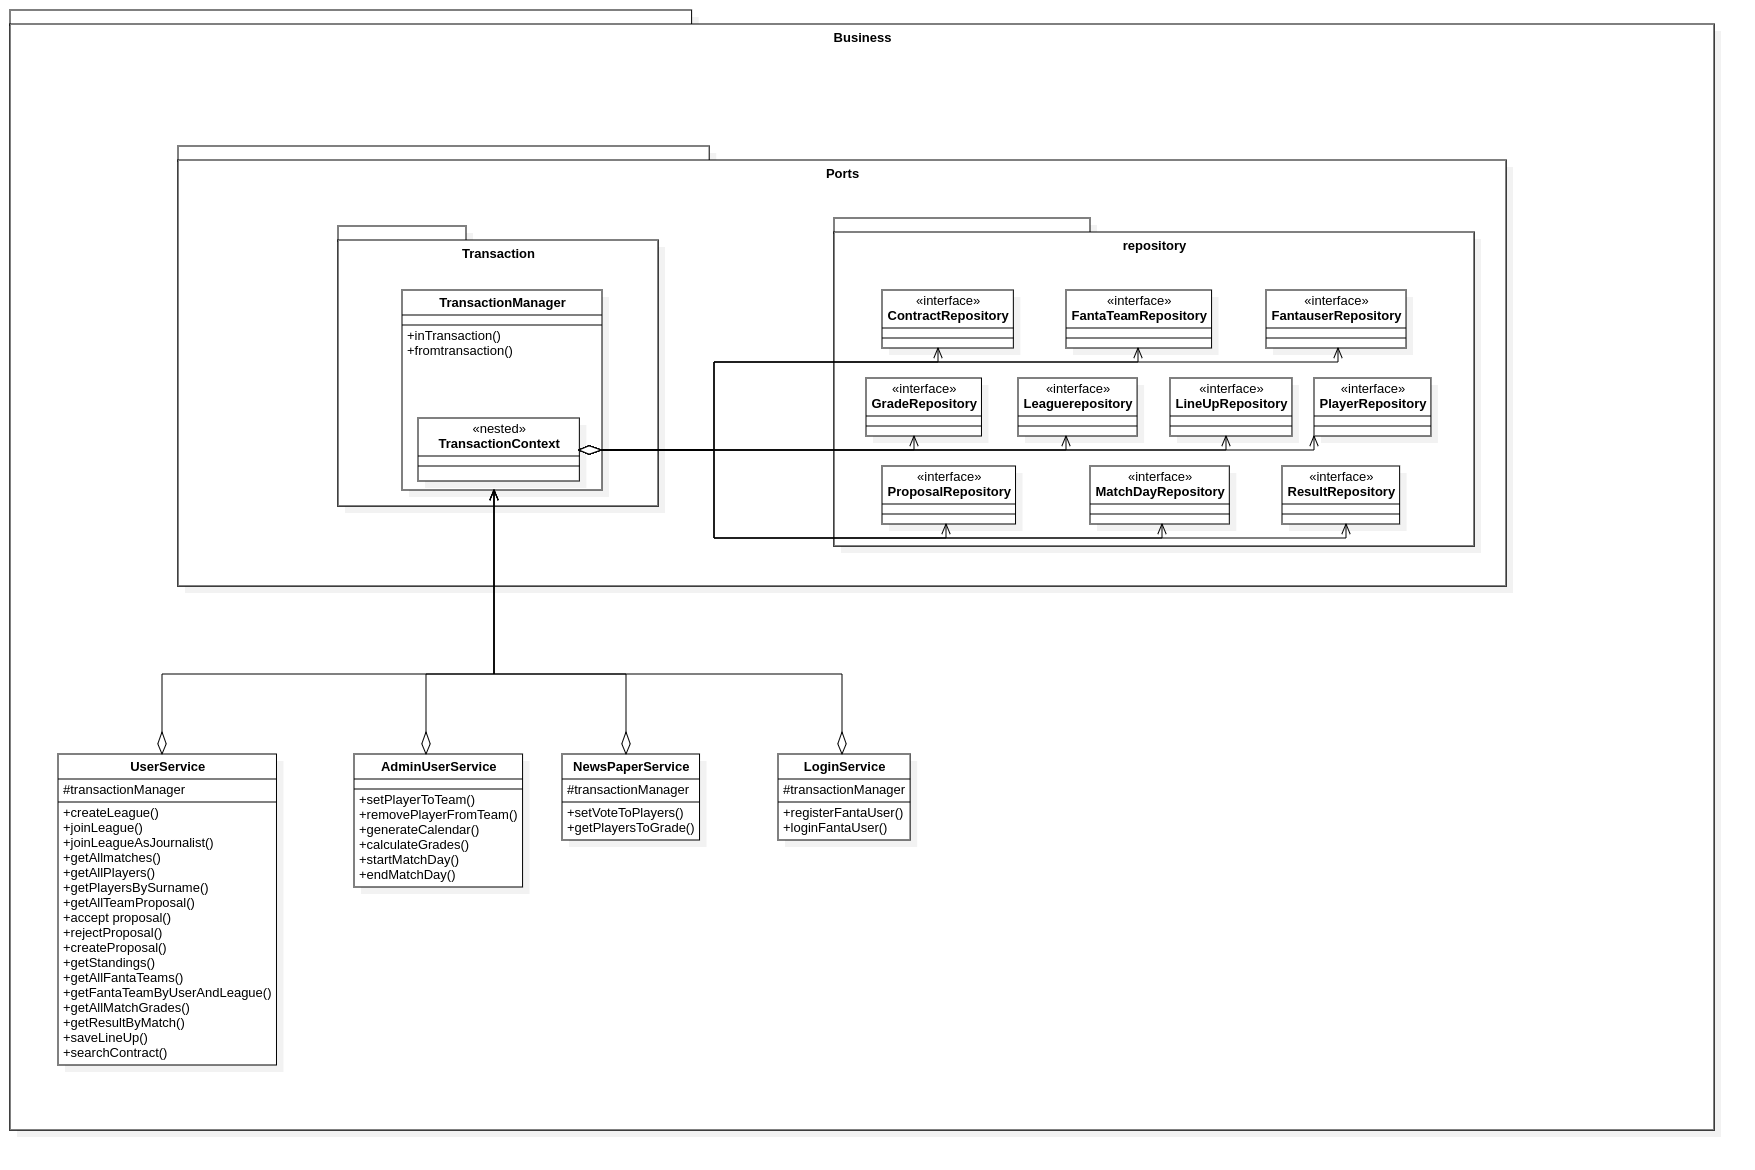
\includegraphics[width=\textwidth]{Resources/graficiUML/BusinessClassDiagram.png}        
    \caption{Business class diagram.}
    \label{fig:business_class_diagram2}
\end{figure}

Di seguito l'implementazione di \textit{inTransaction} e \textit{fromTransaction}:
\begin{lstlisting}[language=Java]
@Override
	public <T> T fromTransaction(Function<TransactionContext, T> code) {

		EntityManager em = emFactory.createEntityManager();
		EntityTransaction transaction = em.getTransaction();
		try {
			transaction.begin();
			T result = code.apply(new TransactionContext(
										new JpaLeagueRepository(em), 
										new JpaMatchRepository(em),
										new JpaPlayerRepository(em), 
										new JpaFantaTeamRepository(em), 
										new JpaGradeRepository(em),
										new JpaProposalRepository(em), 
										new JpaContractRepository(em), 
										new JpaResultsRepository(em),
										new JpaFieldingRepository(em), 
										new JpaLineUpRepository(em), 
										new JpaMatchDayRepository(em),
										new JpaNewsPaperRepository(em), 
										new JpaFantaUserRepository(em)));
			transaction.commit();
			return result;
		} catch (Exception e) {
			if (transaction.isActive()) {
				transaction.rollback();
			}
			throw e;
		} finally {
			em.close();
		}
	}

	@Override
	public void inTransaction(Consumer<TransactionContext> code) {
		fromTransaction((context) -> {
			code.accept(context);
			return true;
		});
	}
}
\end{lstlisting}
\newpage

\subsection{Repositories}
I repository concreti estendono tutti il \textbf{BaseJpaRepository} ed implementano la relativa interfaccia.
Le query sono state implementate con le \textit{CriteriaQuery}, ciò ha permesso insieme
all'utilizzo del metamodello di avere un controllo a compile time sulle entità utilizzate nella query.

\begin{figure}
    \centering
    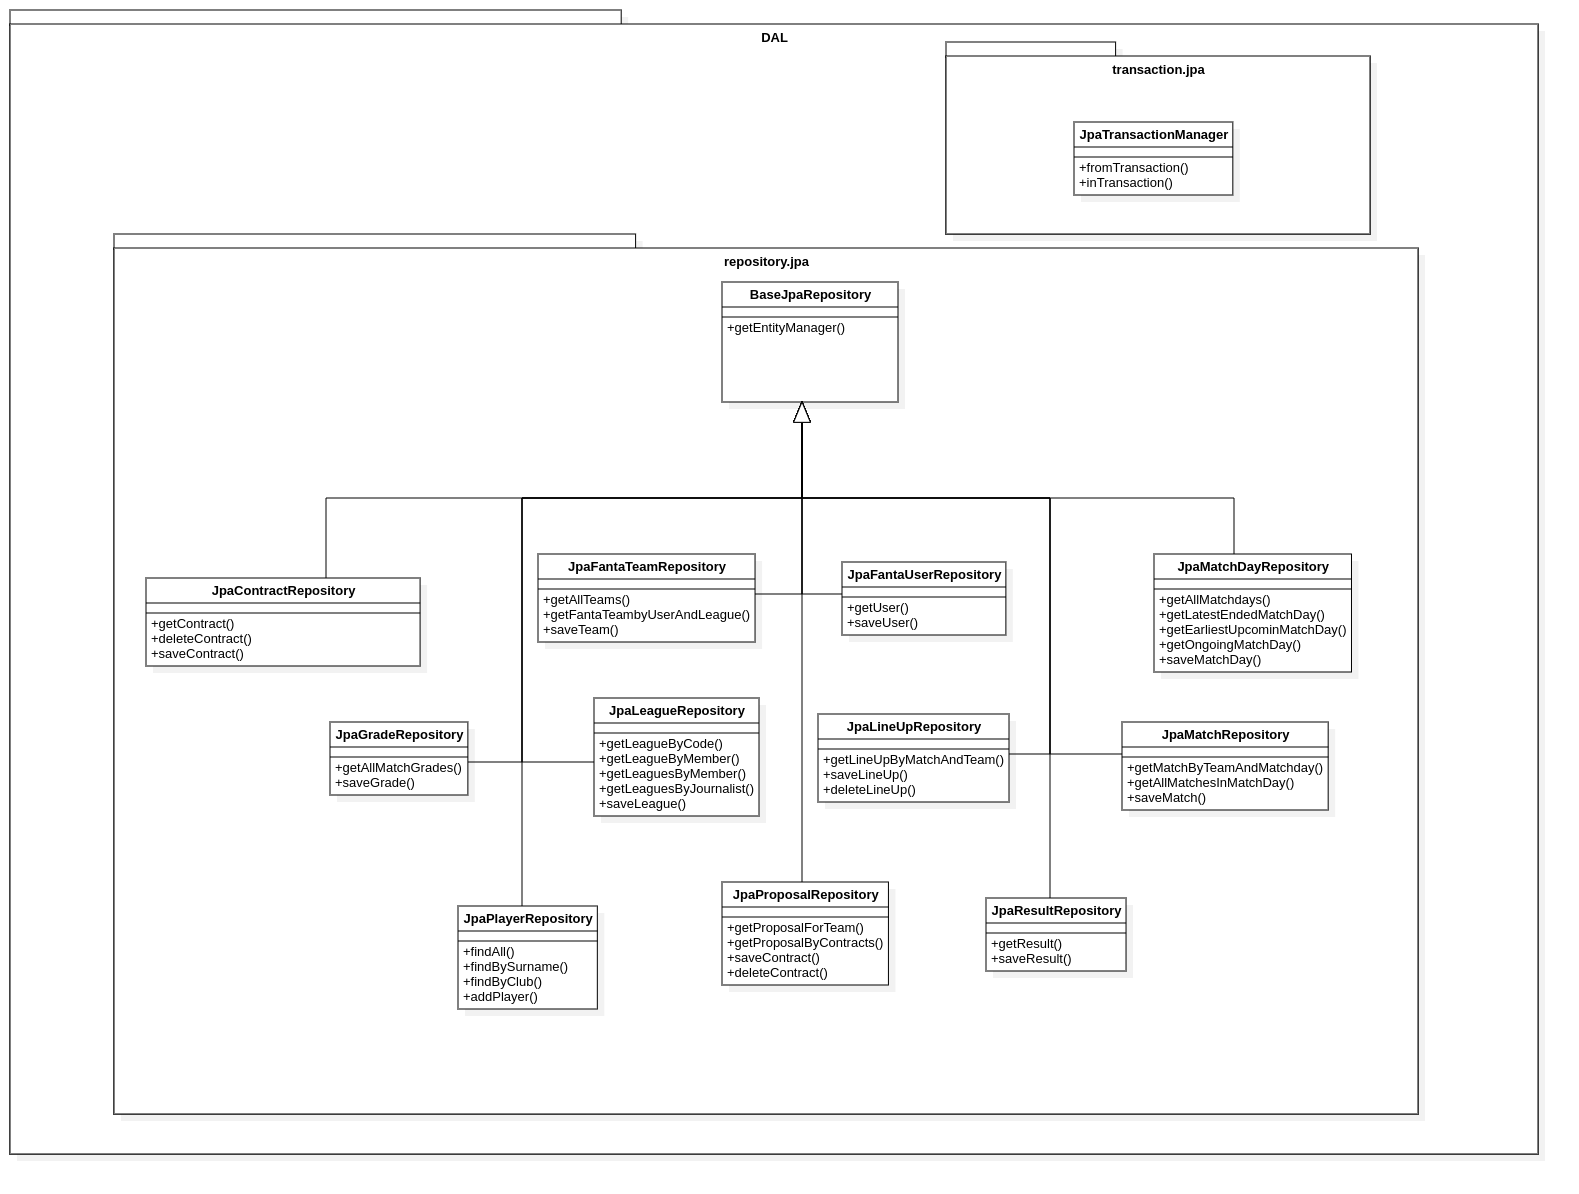
\includegraphics[width=\textwidth]{Resources/graficiUML/DALClassDiagram.png}        
    \caption{Dal class diagram.}
    \label{fig:Dal_class_diagram2}
\end{figure}

Esempio di query effettuata tramite le \textit{CriteriaQuery}:
\begin{lstlisting}[language=Java]
@Override
	public Optional<FantaUser> getUser(String email, String password) {
    	EntityManager em = getEntityManager();
        CriteriaBuilder cb = em.getCriteriaBuilder();
        CriteriaQuery<FantaUser> query = cb.createQuery(FantaUser.class);
        Root<FantaUser> root = query.from(FantaUser.class);

        query.select(root).where(
                cb.equal(root.get(FantaUser_.email), email),
                cb.equal(root.get(FantaUser_.password), password)
        );

        return em.createQuery(query).getResultList().stream().findFirst();
	}
}
\end{lstlisting}

\section{Application Tests}

\subsection{Unit Tests}

I seguenti test verificano il corretto funzionamento delle singole unità di codice.

\subsubsection{Test UT1: Registrazione di un FantaUser} \label{UT1}
\todo{Va tenuto qui?}

Questo unit test verifica il corretto funzionamento del sistema di registrazione di un FantaUser, 
tramite mock dei repository, implementando il template \hyperref[UC-01]{UC-01}.

\begin{lstlisting}[language=Java]
@Test
void testRegisterFantaUser_SavesWhenNotExists() {
    when(fantaUserRepository.getUser("mail", "pswd")).thenReturn(Optional.empty());

    service.registerFantaUser("mail", "pswd");

    verify(fantaUserRepository).saveFantaUser(argThat(user ->
            user.getEmail().equals("mail") && user.getPassword().equals("pswd")));
}
\end{lstlisting}

Similmente sono stati anche prodotti dei test per la registrazione di un NewsPaper.


\subsubsection{Test UT2: Login di un FantaUser} \label{UT2}
\todo{Va tenuto qui?}

Questo unit test verifica il corretto funzionamento del sistema di registrazione di un FantaUser, 
tramite mock dei repository.

\begin{lstlisting}[language=Java]
@Test
void testLoginFantaUser_ReturnsTrueWhenPresent() {
    when(fantaUserRepository.getUser("mail", "pswd"))
            .thenReturn(Optional.of(new FantaUser("mail", "pswd")));

    assertThat(service.loginFantaUser("mail", "pswd")).isTrue();
}
\end{lstlisting}

Similmente sono stati anche prodotti dei test per il login di un NewsPaper.


\subsubsection{Test UT3: Crea fantalega} \label{UT3}

Questo unit test verifica il corretto funzionamento del sistema di creazione di una nuova League,
tramite mock dei repository.

\begin{lstlisting}[language=Java]
@Test
void testCreateLeague() {
	FantaUser admin = new FantaUser("admin@test.com", "pwd");
	NewsPaper np = new NewsPaper("Gazzetta");
	String leagueCode = "L001";

	// League code does not exist yet
	when(leagueRepository.getLeagueByCode(leagueCode))
        .thenReturn(Optional.empty());

	adminUserService.createLeague("My League", admin, np, leagueCode);

	// Verify that saveLeague was called
	verify(leagueRepository, times(1)).saveLeague(any(League.class));
}
\end{lstlisting}


\subsubsection{Test UT4: Genera calendario} \label{UT4}

Questo unit test verifica il corretto funzionamento del sistema di generazione del calendario della League,
tramite mock dei repository.

\begin{lstlisting}[language=Java]
@Test
void testGenerateCalendar_SavesMatches() {
	FantaUser admin = new FantaUser(null, null);
	League league = new League(admin, "Serie A", null, null);

	// Create 4 real teams (even number for round-robin)
	FantaTeam team1 = new FantaTeam("Team1", null, 0, null, new HashSet<>());
	FantaTeam team2 = new FantaTeam("Team2", null, 0, null, new HashSet<>());
	FantaTeam team3 = new FantaTeam("Team3", null, 0, null, new HashSet<>());
	FantaTeam team4 = new FantaTeam("Team4", null, 0, null, new HashSet<>());
	List<FantaTeam> teams = List.of(team1, team2, team3, team4);

	// 38 match days (real objects are okay)
	List<MatchDaySerieA> matchDays = new ArrayList<>();
	for (int i = 0; i < 38; i++)
		matchDays.add(new MatchDaySerieA("match", LocalDate.now()));

	// Mock repositories
	when(fantaTeamRepository.getAllTeams(league)).thenReturn(teams);
	when(matchDayRepository.getAllMatchDays()).thenReturn(matchDays);

	adminUserService.generateCalendar(league);

    verify(matchRepository, atLeastOnce()).saveMatch(any(Match.class));
}
\end{lstlisting}


\subsubsection{Test UT5: Assegna giocatori alle rose} \label{UT5}

Questo unit test verifica il corretto funzionamento del sistema di assegnazione dei Player ai FantaTeam che li hanno acquistati,
tramite mock dei repository.

\begin{lstlisting}[language=Java]
@Test
void testSetPlayerToTeam_SavesContract_WhenBelowLimits() {
	FantaTeam team = new FantaTeam("Team", null, 0, null, new HashSet<>());
	Player.Goalkeeper gk = new Player.Goalkeeper("Gigi", "Buffon", Player.Club.JUVENTUS);

	adminUserService.setPlayerToTeam(team, gk);

	verify(contractRepository).saveContract(argThat(c -> c.getTeam().equals(team) && c.getPlayer().equals(gk)));
}
\end{lstlisting}


\subsubsection{Test UT6: Calcola voti della giornata} \label{UT6}

Questo unit test verifica il corretto funzionamento del sistema di calcolo dei voti della giornata una volta terminata,
tramite mock dei repository.

\begin{lstlisting}[language=Java]
@Test
void testCalculateGrades_SavesResultsAndUpdatesPoints() {

	FantaUser admin = new FantaUser("admin@example.com", "pwd");
	NewsPaper newspaper = new NewsPaper("Gazzetta");
    League league = new League(admin, "Serie A", newspaper, "1234");

	LocalDate matchDate = LocalDate.of(2025, 9, 21); // Sunday
	MatchDaySerieA prevDay = new MatchDaySerieA("Day0", matchDate.minusWeeks(1));
	MatchDaySerieA dayToCalc = new MatchDaySerieA("Day1", matchDate);

	when(matchDayRepository.getPreviousMatchDay(any()))
        .thenReturn(Optional.of(prevDay));

    AdminUserService serviceWithFixedDate = new AdminUserService(transactionManager) {
		@Override
		protected LocalDate today() {
			return matchDate.plusDays(5);
		}

		@Override
		protected Optional<MatchDaySerieA> getNextMatchDayToCalculate(LocalDate d, TransactionContext c, League l,
				FantaUser u) {
			return Optional.of(dayToCalc);
		}
	};

	// Teams
	FantaTeam team1 = new FantaTeam("Team1", league, 0, admin, Set.of());
	FantaTeam team2 = new FantaTeam("Team2", league, 0, admin, Set.of());

	// Match
	Match match = new Match(dayToCalc, team1, team2);
	when(matchRepository.getAllMatchesByMatchDay(dayToCalc, league))
		.thenReturn(List.of(new Match(dayToCalc, team1, team2)));

	// Players
	Player.Goalkeeper gk1 = new Player.Goalkeeper("G1", "Alpha", Player.Club.ATALANTA);
	Player.Goalkeeper gk2 = new Player.Goalkeeper("G2", "Beta", Player.Club.BOLOGNA);

	LineUp lineup1 = new _433LineUp._443LineUpBuilder(match, team1).withGoalkeeper(gk1).build();
	LineUp lineup2 = new _433LineUp._443LineUpBuilder(match, team2).withGoalkeeper(gk2).build();

	when(lineUpRepository.getLineUpByMatchAndTeam(match, team1)).thenReturn(Optional.of(lineup1));
	when(lineUpRepository.getLineUpByMatchAndTeam(match, team2)).thenReturn(Optional.of(lineup2));

	// Grades
	Grade grade1 = new Grade(gk1, dayToCalc, 70.0, newspaper);
	Grade grade2 = new Grade(gk2, dayToCalc, 60.0, newspaper);
	when(gradeRepository.getAllMatchGrades(match, newspaper)).thenReturn(List.of(grade1, grade2));

	// Act
	serviceWithFixedDate.calculateGrades(admin, league);

	// Assert: Result persisted
	verify(resultRepository).saveResult(any());

	// Assert: team points updated
	assertThat(team1.getPoints()).isEqualTo(3);
	assertThat(team2.getPoints()).isEqualTo(0);
}
\end{lstlisting}


\subsubsection{Test UT7: Unisciti alla lega} \label{UT7}

Questo unit test verifica il corretto funzionamento del sistema di ingresso in una League,
tramite mock dei repository.

\begin{lstlisting}[language=Java]
@Test
void testJoinLeague() {
	FantaUser user = new FantaUser("user@test.com", "pwd");
	League league = new League(user, "Test League", new NewsPaper("Gazzetta"), "L002");
	FantaTeam team = new FantaTeam("Team A", league, 0, user, Set.of());

	when(leagueRepository.getLeaguesByUser(user))
        .thenReturn(Collections.emptyList());

	userService.joinLeague(team, league);

	verify(teamRepository, times(1)).saveTeam(team);
}
\end{lstlisting}


\subsubsection{Test UT8: Visualizza calendario} \label{UT8}

Questo unit test verifica il corretto funzionamento del sistema di visualizzazione del calendario,
tramite mock dei repository.

\begin{lstlisting}[language=Java]
@Test
void testGetAllMatches() {
	League league = new League(null, null, null, null);
	MatchDaySerieA day1 = new MatchDaySerieA(null, null);
	Match m1 = new Match(day1, null, null);
	when(context.getMatchDayRepository().getAllMatchDays())
        .thenReturn(List.of(day1));
	when(context.getMatchRepository().getAllMatchesByMatchDay(day1, league))
        .thenReturn(List.of(m1));

	Map<MatchDaySerieA, List<Match>> result = userService.getAllMatches(league);
	assertThat(result.get(day1)).containsExactly(m1);
	}
\end{lstlisting}


\subsubsection{Test UT9: Inserisci formazione} \label{UT9}

Questo unit test verifica il corretto funzionamento del sistema di salvataggio della LineUp,
tramite mock dei repository.

\begin{lstlisting}[language=Java]
@Test
void testSaveLineUp() {
	FantaUser user = new FantaUser("user@test.com", "pwd");
	League league = new League(user, "Test League", new NewsPaper("Gazzetta"), "L003");
	MatchDaySerieA matchDay = new MatchDaySerieA("MD1", LocalDate.of(2025, 9, 15)); // Monday
	FantaTeam team = new FantaTeam("Dream Team", league, 30, user, new HashSet<>());
	Match match = new Match(matchDay, team, team);
	LineUp lineUp = new _433LineUp._443LineUpBuilder(match, team).build();

	UserService spyService = spy(userService);
	doReturn(team).when(spyService).getFantaTeamByUserAndLeague(league, user);
	doReturn(LocalDate.of(2025, 9, 15)).when(spyService).today(); // Current Monday

	// Stub repos
	when(context.getMatchDayRepository().getPreviousMatchDay(any()))
        .thenReturn(Optional.empty());
	when(context.getLineUpRepository().getLineUpByMatchAndTeam(match, team))
        .thenReturn(Optional.empty());

	spyService.saveLineUp(lineUp);

	verify(context.getLineUpRepository()).saveLineUp(lineUp);
}
\end{lstlisting}


\subsubsection{Test UT10: Visualizza prossimo Match} \label{UT10}

Questo unit test verifica il corretto funzionamento del sistema di visualizzazione del prossimo Match,
tramite mock dei repository.

\begin{lstlisting}[language=Java]
@Test
void testGetNextMatch() {
    League league = new League(null, null, null, null);
	FantaTeam team = new FantaTeam(null, league, 0, null, null);
	MatchDaySerieA prev = new MatchDaySerieA(null, null);
	MatchDaySerieA next = new MatchDaySerieA(null, null);
	Match prevMatch = new Match(next, team, team);
	Match nextMatch = new Match(next, team, team);

	when(context.getMatchDayRepository().getPreviousMatchDay(any()))
        .thenReturn(Optional.of(prev));
	when(context.getMatchRepository().getMatchByMatchDay(prev, league, team))
        .thenReturn(prevMatch);
	when(resultRepository.getResult(prevMatch))
        .thenReturn(Optional.of(mock(Result.class)));
	when(context.getMatchDayRepository().getNextMatchDay(any()))
        .thenReturn(Optional.of(next));
	when(context.getMatchRepository().getMatchByMatchDay(next, league, team))
        .thenReturn(nextMatch);

	Match result = userService.getNextMatch(league, team, LocalDate.now());
	assertThat(result).isEqualTo(nextMatch);
}
\end{lstlisting}


\subsubsection{Test UT11: Visualizza classifica} \label{UT11}

Questo unit test verifica il corretto funzionamento del sistema di visualizzazione della classifica,
tramite mock dei repository.

\begin{lstlisting}[language=Java]
@Test
void testGetStandings() {
	League league = new League(null, null, null, null);
	FantaTeam t1 = mock(FantaTeam.class);
	FantaTeam t2 = mock(FantaTeam.class);

	when(t1.getPoints()).thenReturn(10);
	when(t2.getPoints()).thenReturn(20);

	UserService spyService = spy(userService);
	doReturn(List.of(t1, t2)).when(spyService).getAllFantaTeams(league);

	List<FantaTeam> standings = spyService.getStandings(league);

	assertThat(standings).containsExactly(t2, t1);
}
\end{lstlisting}


\subsubsection{Test UT12: Scambia giocatori - Invia proposta} \label{UT12}

Questo unit test verifica il corretto funzionamento del sistema di invio di proposte di scambio di Player tra due FantaTeam
tramite mock dei repository.

\begin{lstlisting}[language=Java]
@Test
void testCreateProposal_HappyPath() {
	League league = new League(null, null, null, null);
	FantaUser user = new FantaUser(null, null);
	FantaTeam myTeam = spy(new FantaTeam("My Team", league, 0, user, new HashSet<>()));
	FantaTeam opponentTeam = new FantaTeam("Opponent", league, 0, user, new HashSet<>());
	Player offeredPlayer = new Player.Defender(null, null, null);
	Player requestedPlayer = new Player.Defender(null, null, null);

	Contract offeredContract = new Contract(myTeam, offeredPlayer);
	Contract requestedContract = new Contract(opponentTeam, requestedPlayer);
	myTeam.getContracts().add(offeredContract);
	opponentTeam.getContracts().add(requestedContract);

	when(context.getProposalRepository().getProposal(offeredContract, requestedContract))
		.thenReturn(Optional.empty());
	when(context.getProposalRepository().saveProposal(any()))
        .thenReturn(true);

	assertThat(userService.createProposal(requestedPlayer, offeredPlayer, myTeam, opponentTeam)).isTrue();
}
\end{lstlisting}


\subsubsection{Test UT13: Scambia giocatori - Accetta proposta} \label{UT13}

Questo unit test verifica il corretto funzionamento del sistema di accettazione di una proposta di scambio di Player 
tramite mock dei repository.

\begin{lstlisting}[language=Java]
@Test
void testAcceptProposal() {
	// Setup teams and players
	FantaTeam myTeam = mock(FantaTeam.class);
	FantaTeam offeringTeam = new FantaTeam(null, null, 0, null, null);
	Player offeredPlayer = new Player.Forward(null, null, null);
	Player requestedPlayer = new Player.Midfielder(null, null, null);

	// Contracts
	Contract offeredContract = mock(Contract.class);
	when(offeredContract.getTeam()).thenReturn(offeringTeam);
	when(offeredContract.getPlayer()).thenReturn(offeredPlayer);

    Contract requestedContract = mock(Contract.class);
    when(requestedContract.getTeam()).thenReturn(myTeam);
	when(requestedContract.getPlayer()).thenReturn(requestedPlayer);

	// Proposal
	Proposal.PendingProposal proposal = mock(Proposal.PendingProposal.class);
	when(proposal.getRequestedContract()).thenReturn(requestedContract);
	when(proposal.getOfferedContract()).thenReturn(offeredContract);

	// Stub isSameTeam
	when(myTeam.isSameTeam(myTeam)).thenReturn(true);

	// Stub searchContract to return non-empty Optionals
	UserService userServiceSpy = spy(userService);
	doReturn(Optional.of(requestedContract))
        .when(userServiceSpy).searchContract(myTeam, requestedPlayer);
	doReturn(Optional.of(offeredContract))
        .when(userServiceSpy).searchContract(offeringTeam, offeredPlayer);

	// Run test
	userServiceSpy.acceptProposal(proposal, myTeam);

	// Verify repository interactions
	verify(context.getContractRepository())
        .deleteContract(requestedContract);
	verify(context.getContractRepository())
        .deleteContract(offeredContract);
	verify(context.getContractRepository(), times(2)).saveContract(any(Contract.class));
	verify(context.getProposalRepository()).deleteProposal(proposal);
}
\end{lstlisting}


\subsubsection{Test UT14: Visualizza squadre} \label{UT14}

Questo unit test verifica il corretto funzionamento del sistema di visualizzazione di tutti i FantaTeam 
tramite mock dei repository.

\begin{lstlisting}[language=Java]
@Test
void testGetAllFantaTeams() {
    League league = new League(null, "My League", new NewsPaper("Gazzetta"), "L999");
	FantaTeam t1 = new FantaTeam("Team 1", league, 0, new FantaUser("u1", "pwd"), Set.of());
	FantaTeam t2 = new FantaTeam("Team 2", league, 0, new FantaUser("u2", "pwd"), Set.of());

	when(context.getTeamRepository().getAllTeams(league))
        .thenReturn(List.of(t1, t2));

	List<FantaTeam> result = userService.getAllFantaTeams(league);

	assertThat(result).containsExactly(t1, t2);
	verify(context.getTeamRepository(), times(1)).getAllTeams(league);
}
\end{lstlisting}


\subsubsection{Test UT15: Visualizza listone giocatori} \label{UT15}

Questo unit test verifica il corretto funzionamento del sistema di visualizzazione di tutti i giocatori 
tramite mock dei repository.

\begin{lstlisting}[language=Java]
@Test
void testGetAllPlayers() {
	Player p1 = new Player.Goalkeeper("", "", null);
	Player p2 = new Player.Goalkeeper("", "", null);
	when(context.getPlayerRepository().findAll()).thenReturn(List.of(p1, p2));

	List<Player> result = userService.getAllPlayers();
	assertThat(result).containsExactly(p1, p2);
}
\end{lstlisting}


\subsubsection{Test UT16: Assegna voti ai giocatori} \label{UT16}

Questo unit test verifica il corretto funzionamento del sistema di assegnazione dei voti ai Player tramite mock dei repository.

\begin{lstlisting}[language=Java]
@Test
void testSetVoteToPlayers_MultipleGrades() {
	Grade grade2 = mock(Grade.class);
	when(grade2.getMatchDay()).thenReturn(matchDay);
	when(grade2.getMark()).thenReturn(15.0);

	NewsPaperService spyService = spy(service);
	doReturn(Optional.of(matchDay)).when(spyService).getMatchDay();

	spyService.setVoteToPlayers(Set.of(grade, grade2));

	verify(gradeRepository).saveGrade(grade);
	verify(gradeRepository).saveGrade(grade2);
}
\end{lstlisting}


\subsubsection{Test relativi ai JpaRepositories}

Per ogni repository implementata tramite JPA è stata realizzata una classe di test per verificare la 
corretta interazione con il database, sia per salvare nuovi elementi, sia per recuperare dati. 
Di seguito è proposto un test che verifica il corretto salvataggio nel database di un nuovo FantaTeam.

\begin{lstlisting}[language=Java]
@Test
@DisplayName("saveTeam() should persist correctly")
public void testSaveTeam() {

	entityManager.getTransaction().begin();

	FantaUser user = new FantaUser("mail1", "pswd1");
	FantaTeam team = new FantaTeam("team1", league, 0, user, new HashSet<Contract>());

	entityManager.persist(user);

	fantaTeamRepository.saveTeam(team);

	FantaTeam result = entityManager
		.createQuery("FROM FantaTeam t WHERE t.league = :league AND t.fantaManager = :user", FantaTeam.class)
		.setParameter("league", league).setParameter("user", user).getSingleResult();

	assertThat(result).isEqualTo(team);

    entityManager.close();
}
\end{lstlisting}

Di seguito è invece proposto un test che verifica che il recupero di informazioni dal database sia corretto: 
in particolare, l'obiettivo è recuperare tutti i voti assegnati in un singolo match.

\begin{lstlisting}[language=Java]
@Test
@DisplayName("getAllMatchGrades() when two grades have been persisted")
public void testGetAllMatchGradesWhenTwoGradesExist() {
	Player player1 = new Player.Goalkeeper("Gigi", "Buffon", Club.JUVENTUS);
	Player player2 = new Player.Forward("Gigi", "Riva", Club.CAGLIARI);

    Grade voto1 = new Grade(player1, matchDay, 6.0, newsPaper);
	Grade voto2 = new Grade(player1, matchDay, 8.0, newsPaper);
	Contract contract1 = new Contract(team1, player1);
	Contract contract2 = new Contract(team1, player2);
	sessionFactory.inTransaction(session -> {
		session.persist(player1);
		session.persist(player2);
		session.persist(voto1);
		session.persist(voto2);
		session.persist(contract1);
		session.persist(contract2);
	});

	assertThat(gradeRepository.getAllMatchGrades(match, newsPaper)).containsExactly(voto1, voto2);
}
\end{lstlisting}


\subsubsection{Test relativi al Domain Model}

Inoltre, sono stati creati degli unit test per verificare il corretto comportamento di alcuni metodi presenti nelle classi del Domain Model:
\begin{itemize}
    \item la classe \textit{\_433LineUp} usa il pattern \textbf{Builder}, perciò si testa che la costruzione di nuovi oggetti sia corretta;
    \item la classe \textit{FantaTeamViewer}, sfruttando il pattern \textbf{Visitor}, si occupa di recuperare gli 
        insiemi di giocatori appartenenti ad un FantaTeam divisi per ruoli basandosi sui contratti del FantaTeam;
    \item la classe \textit{LineUpViewer}, similmente a \textit{FantaTeamViewer}, si occupa di recuperare gli 
        insiemi di giocatori presenti in una LineUp divisi per ruoli.
\end{itemize}



\subsection{Integration Tests}

I seguenti test verificano che le varie componenti cooperino correttamente per l'implementazione degli use case richiesti.


\subsubsection{Test IT1: Crea fantalega} \label{IT1}

Questo unit test verifica il corretto funzionamento del sistema di creazione di una nuova League,
implementando il template \hyperref[UC-01]{UC-01}.

\begin{lstlisting}[language=Java]
@Test
void createLeague() {

	entityManager.getTransaction().begin();

	FantaUser admin = new FantaUser("mail", "pswd");
	fantaUserRepository.saveFantaUser(admin);

	NewsPaper newsPaper = new NewsPaper("Gazzetta");
	newspaperRepository.saveNewsPaper(newsPaper);

	entityManager.getTransaction().commit();

	adminUserService.createLeague("lega", admin, newsPaper, "1234");

    Optional<League> result = leagueRepository.getLeagueByCode("1234");

	assertThat(result.isPresent());
	League league = result.get();

	assertThat(league.getName()).isEqualTo("lega");
	assertThat(league.getAdmin()).isEqualTo(admin);
	assertThat(league.getNewsPaper()).isEqualTo(newsPaper);
	assertThat(league.getLeagueCode()).isEqualTo("1234");
}
\end{lstlisting}

\begin{comment}
\subsubsection{Test IT4: Genera calendario} \label{IT4}

Questo unit test verifica il corretto funzionamento del sistema di generazione del calendario della League,
implementando il template XXXXXXXX \todo{collegare al template}.

\begin{lstlisting}[language=Java]
@Test
void generateCalendar() {

	entityManager.getTransaction().begin();

	FantaUser admin = new FantaUser("mail", "pswd");
	FantaUser user = new FantaUser("user2", "pswd2");
	fantaUserRepository.saveFantaUser(admin);
	fantaUserRepository.saveFantaUser(user);

	NewsPaper newsPaper = new NewsPaper("Gazzetta");
	newspaperRepository.saveNewsPaper(newsPaper);

	League league = new League(admin, "lega", newsPaper, "0000");
	leagueRepository.saveLeague(league);

	FantaTeam team1 = new FantaTeam("team1", league, 0, admin, new HashSet<Contract>());
	FantaTeam team2 = new FantaTeam("team2", league, 0, user, new HashSet<Contract>());

	fantaTeamRepository.saveTeam(team1);
	fantaTeamRepository.saveTeam(team2);

	List<MatchDaySerieA> matchDays = new ArrayList<MatchDaySerieA>();
	for (int i = 0; i < 38; i++) {
		matchDays.add(new MatchDaySerieA("Match " + String.valueOf(i), LocalDate.of(2025, 9, 7).plusWeeks(i)));
	}

    sessionFactory.inTransaction(t -> {
		for (MatchDaySerieA matchDaySerieA : matchDays) {
			t.persist(matchDaySerieA);
		}
	});

	entityManager.getTransaction().commit();

    adminUserService.generateCalendar(league);

	for (MatchDaySerieA matchDaySerieA : matchDays) {
		Match matchByMatchDay = matchRepository.getMatchByMatchDay(matchDaySerieA, league, team1);

		assertThat(matchByMatchDay.getMatchDaySerieA()).isEqualTo(matchDaySerieA);
		assertThat(matchByMatchDay.getTeam1().equals(team1) || matchByMatchDay.getTeam2().equals(team1)).isTrue();
	}
}
\end{lstlisting}

\end{comment}

\subsubsection{Test IT2: Assegna giocatori alle rose} \label{IT2}

Questo unit test verifica il corretto funzionamento del sistema di assegnazione dei Player ai FantaTeam che li hanno acquistati,
implementando il template \hyperref[UC-02]{UC-02}.

\begin{lstlisting}[language=Java]
@Test
void setPlayersToTeam() {

	entityManager.getTransaction().begin();

    FantaUser admin = new FantaUser("mail", "pswd");
	fantaUserRepository.saveFantaUser(admin);

    NewsPaper newsPaper = new NewsPaper("Gazzetta");
	newspaperRepository.saveNewsPaper(newsPaper);

    League league = new League(admin, "lega", newsPaper, "1234");
	leagueRepository.saveLeague(league);

	FantaTeam team = new FantaTeam("", league, 0, admin, Set.of());
	fantaTeamRepository.saveTeam(team);

	Player.Forward player = new Player.Forward("Lionel", "Messi", Club.CREMONESE);
	Player.Goalkeeper player2 = new Player.Goalkeeper("Gigi", "Buffon", Club.JUVENTUS);
	playerRepository.addPlayer(player);
	playerRepository.addPlayer(player2);

	entityManager.getTransaction().commit();

	adminUserService.setPlayerToTeam(team, player);
	adminUserService.setPlayerToTeam(team, player2);

	Optional<Contract> contract = contractRepository.getContract(team, player);
	assertThat(contract).isPresent();
	Contract found = contract.get();
	assertThat(found.getPlayer()).isEqualTo(player);
	assertThat(found.getTeam()).isEqualTo(team);

    Optional<Contract> contract2 = contractRepository.getContract(team, player);
	assertThat(contract2).isPresent();
	Contract found2 = contract.get();
	assertThat(found2.getPlayer()).isEqualTo(player);
	assertThat(found2.getTeam()).isEqualTo(team);

}
\end{lstlisting}


\begin{comment}
\subsubsection{Test IT6: Calcola voti della giornata} \label{IT6}

Questo unit test verifica il corretto funzionamento del sistema di calcolo dei voti della giornata una volta terminata,
implementando il template XXXXXXXX \todo{collegare al template}.

\begin{lstlisting}[language=Java]
@Test
void calculateGrades() {

	entityManager.getTransaction().begin();

	// Users
	FantaUser admin = new FantaUser("mail", "pswd");
	FantaUser user = new FantaUser("mail2", "pswd2");

	fantaUserRepository.saveFantaUser(admin);
	fantaUserRepository.saveFantaUser(user);

	NewsPaper newsPaper = new NewsPaper("Gazzetta");
	newspaperRepository.saveNewsPaper(newsPaper);

	League league = new League(admin, "lega", newsPaper, "0000");
	leagueRepository.saveLeague(league);

	// Teams
	FantaTeam team1 = new FantaTeam("team1", league, 0, admin, new HashSet<Contract>());
	FantaTeam team2 = new FantaTeam("team2", league, 0, user, new HashSet<Contract>());

	fantaTeamRepository.saveTeam(team1);
	fantaTeamRepository.saveTeam(team2);

	// MatchDays
	LocalDate matchDate = LocalDate.of(2025, 9, 14);
	MatchDaySerieA prevDay = new MatchDaySerieA("Day0", matchDate.minusWeeks(1));
	MatchDaySerieA dayToCalc = new MatchDaySerieA("Day1", matchDate);

	entityManager.persist(prevDay);
	entityManager.persist(dayToCalc);

	// Match
	Match prevMatch = new Match(prevDay, team1, team2);
	Match match = new Match(dayToCalc, team1, team2);

	matchRepository.saveMatch(prevMatch);
	matchRepository.saveMatch(match);

	// Players
	Goalkeeper gk1 = new Goalkeeper("Gianluigi", "Buffon", Club.JUVENTUS);
	Goalkeeper gk2 = new Goalkeeper("Samir", "Handanovic", Club.INTER);

	Defender d1 = new Defender("Paolo", "Maldini", Club.MILAN);
	Defender d2 = new Defender("Franco", "Baresi", Club.JUVENTUS);
	Defender d3 = new Defender("Alessandro", "Nesta", Club.LAZIO);
	Defender d4 = new Defender("Giorgio", "Chiellini", Club.JUVENTUS);
	Defender d5 = new Defender("Leonardo", "Bonucci", Club.JUVENTUS);

	Midfielder m1 = new Midfielder("Andrea", "Pirlo", Club.JUVENTUS);
    Midfielder m2 = new Midfielder("Daniele", "De Rossi", Club.ROMA);
	Midfielder m3 = new Midfielder("Marco", "Verratti", Club.CREMONESE);
	Midfielder m4 = new Midfielder("Claudio", "Marchisio", Club.JUVENTUS);

	Forward f1 = new Forward("Roberto", "Baggio", Club.BOLOGNA);
	Forward f2 = new Forward("Francesco", "Totti", Club.ROMA);
	Forward f3 = new Forward("Alessandro", "Del Piero", Club.JUVENTUS);
	Forward f4 = new Forward("Lorenzo", "Insigne", Club.NAPOLI);

	List<Player> players = List.of(gk1, gk2, d1, d2, d3, d4, d5, m1, m2, m3, m4, f1, f2, f3, f4);

	players.forEach(playerRepository::addPlayer);

	for (Player player : players) {
		contractRepository.saveContract(new Contract(team1, player));
		contractRepository.saveContract(new Contract(team2, player));
	}

	// LineUps
	LineUp lineup1 = new _433LineUp._443LineUpBuilder(match, team1).withGoalkeeper(gk1)
			.withDefenders(d1, d2, d3, d4).withMidfielders(m1, m2, m3).withForwards(f1, f2, f3)
			.withSubstituteGoalkeepers(List.of(gk2)).withSubstituteDefenders(List.of(d5))
			.withSubstituteMidfielders(List.of(m4)).withSubstituteForwards(List.of(f4)).build();
	LineUp lineup2 = new _433LineUp._443LineUpBuilder(match, team2).withGoalkeeper(gk1)
			.withDefenders(d1, d2, d3, d4).withMidfielders(m1, m2, m3).withForwards(f1, f2, f3)
			.withSubstituteGoalkeepers(List.of(gk2)).withSubstituteDefenders(List.of(d5))
			.withSubstituteMidfielders(List.of(m4)).withSubstituteForwards(List.of(f4)).build();

	lineUpRepository.saveLineUp(lineup1);
	lineUpRepository.saveLineUp(lineup2);

	// Grades
	Grade grade1 = new Grade(gk1, dayToCalc, 70.0, newsPaper);
	Grade grade2 = new Grade(gk2, dayToCalc, 60.0, newsPaper);

	gradeRepository.saveGrade(grade1);
	gradeRepository.saveGrade(grade2);

	entityManager.getTransaction().commit();

	AdminUserService service = new AdminUserService(transactionManager) {
		@Override
		protected LocalDate today() {
			return LocalDate.of(2025, 9, 16); // after 14/09
		}
	};

	service.calculateGrades(admin, league);

	List<Grade> allMatchGrades = gradeRepository.getAllMatchGrades(match, newsPaper);
	assertThat(allMatchGrades.size()).isEqualTo(2);
	assertThat(allMatchGrades.get(0)).isEqualTo(grade1);
	assertThat(allMatchGrades.get(1)).isEqualTo(grade2);

}
\end{lstlisting}


\subsubsection{Test IT7: Unisciti alla lega} \label{IT7}

Questo unit test verifica il corretto funzionamento del sistema di ingresso in una League,
implementando il template XXXXXXXX \todo{collegare al template}.

\begin{lstlisting}[language=Java]
@Test
void joinLeague() {

	entityManager.getTransaction().begin();
	
	FantaUser user = new FantaUser("user@test.com", "pwd");
	fantaUserRepository.saveFantaUser(user);
		
	NewsPaper newsPaper = new NewsPaper("Gazzetta");
	newspaperRepository.saveNewsPaper(newsPaper);
		
	League league = new League(user, "Test League", newsPaper, "1234");
	leagueRepository.saveLeague(league);
		
	FantaTeam team = new FantaTeam("Team A", league, 0, user, new HashSet<Contract>());

	entityManager.getTransaction().commit();
		
	userService.joinLeague(team, league);
		
	Optional<League> result = leagueRepository.getLeagueByCode("1234");
	assertThat(result).isPresent();
		
	League resultLeague = result.get();
	assertThat(resultLeague.getAdmin()).isEqualTo(user);
	assertThat(resultLeague.getLeagueCode()).isEqualTo("1234");
	assertThat(resultLeague.getName()).isEqualTo("Test League");
	assertThat(resultLeague.getNewsPaper()).isEqualTo(newsPaper);
}
\end{lstlisting}


\subsubsection{Test IT8: Visualizza calendario} \label{IT8}

Questo unit test verifica il corretto funzionamento del sistema di visualizzazione del calendario, cioè della lista dei Match,
implementando il template XXXXXXXX \todo{collegare al template}.

\begin{lstlisting}[language=Java]
@Test
void testGetAllMatches() {
		
	entityManager.getTransaction().begin();
		
	FantaUser user1 = new FantaUser("user1@test.com", "pwd");
	fantaUserRepository.saveFantaUser(user1);
	FantaUser user2 = new FantaUser("user2@test.com", "pwd");
	fantaUserRepository.saveFantaUser(user2);
		
	NewsPaper newsPaper = new NewsPaper("Gazzetta");
	newspaperRepository.saveNewsPaper(newsPaper);
		
	League league = new League(user1, "Test League", newsPaper, "1234");
	leagueRepository.saveLeague(league);
		
	FantaTeam team1 = new FantaTeam("Team A", league, 0, user1, new HashSet<Contract>());
	fantaTeamRepository.saveTeam(team1);
	FantaTeam team2 = new FantaTeam("Team B", league, 0, user2, new HashSet<Contract>());
	fantaTeamRepository.saveTeam(team2);
		
	MatchDaySerieA day1 = new MatchDaySerieA("MD1", LocalDate.of(2025, 9, 7));
	matchDayRepository.saveMatchDay(day1);
		
	Match m1 = new Match(day1, team1, team2);
	matchRepository.saveMatch(m1);
		
	entityManager.getTransaction().commit();
		
	Map<MatchDaySerieA, List<Match>> result = userService.getAllMatches(league);		
		
	assertThat(result.get(day1).size()).isEqualTo(1);
	Match resultMatch = result.get(day1).get(0);
		
	assertThat(resultMatch.getMatchDaySerieA().getName()).isEqualTo("MD1");
}
\end{lstlisting}

\end{comment}

\subsubsection{Test IT3: Inserisci formazione} \label{IT3}

Questo unit test verifica il corretto funzionamento del sistema di salvataggio della LineUp,
implementando il template \hyperref[UC-03]{UC-03}.

\begin{lstlisting}[language=Java]
@Test
void testSaveLineUp() {
		
	entityManager.getTransaction().begin();
		
	FantaUser user = new FantaUser("user@test.com", "pwd");
	fantaUserRepository.saveFantaUser(user);
		
	NewsPaper newsPaper = new NewsPaper("Gazzetta");
	newspaperRepository.saveNewsPaper(newsPaper);
		
	League league = new League(user, "Test League", newsPaper, "L003");
	leagueRepository.saveLeague(league);
		
	MatchDaySerieA matchDay = new MatchDaySerieA("MD1", LocalDate.now().plusWeeks(1)); // Monday
	matchDayRepository.saveMatchDay(matchDay);
		
	FantaTeam team = new FantaTeam("Dream Team", league, 30, user, new HashSet<>());
	fantaTeamRepository.saveTeam(team);
		
	Match match = new Match(matchDay, team, team);
	matchRepository.saveMatch(match);
		
	LineUp lineUp = new _433LineUp._443LineUpBuilder(match, team).build();
		
	entityManager.getTransaction().commit();
		
	userService.saveLineUp(lineUp);
		
	Optional<LineUp> result = lineUpRepository.getLineUpByMatchAndTeam(match, team);
	assertThat(result).isPresent();
		
	LineUp resultLineUp = result.get();
	assertThat(resultLineUp.getMatch()).isEqualTo(match);
	assertThat(resultLineUp.getTeam()).isEqualTo(team);
		
}
\end{lstlisting}

\begin{comment}

\subsubsection{Test IT10: Visualizza prossimo Match} \label{IT10}

Questo unit test verifica il corretto funzionamento del sistema di visualizzazione del prossimo Match,
implementando il template XXXXXXXX \todo{collegare al template}.

\begin{lstlisting}[language=Java]
@Test
void testGetNextMatch() {

	entityManager.getTransaction().begin();

	FantaUser user = new FantaUser("user@test.com", "pwd");
	fantaUserRepository.saveFantaUser(user);

	NewsPaper newsPaper = new NewsPaper("Gazzetta");
	newspaperRepository.saveNewsPaper(newsPaper);

	League league = new League(user, "Test League", newsPaper, "L003");
	leagueRepository.saveLeague(league);

	FantaTeam team = new FantaTeam("Team", league, 30, user, new HashSet<>());
	FantaTeam team2 = new FantaTeam("Team2", league, 40, user, new HashSet<>());
	fantaTeamRepository.saveTeam(team);
	fantaTeamRepository.saveTeam(team2);

	MatchDaySerieA prevMatchDay = new MatchDaySerieA("MD1", LocalDate.now().minusWeeks(1));
	MatchDaySerieA nextMatchDay = new MatchDaySerieA("MD2", LocalDate.now().plusWeeks(1));
	matchDayRepository.saveMatchDay(prevMatchDay);
	matchDayRepository.saveMatchDay(nextMatchDay);

	Match prevMatch = new Match(prevMatchDay, team, team2);
	Match nextMatch = new Match(nextMatchDay, team, team2);
	matchRepository.saveMatch(prevMatch);
	matchRepository.saveMatch(nextMatch);

	Result prevResults = new Result(20, 50, 1, 2, prevMatch);
	resultsRepository.saveResult(prevResults);

	entityManager.getTransaction().commit();

	Match result = userService.getNextMatch(league, team, LocalDate.now());
	assertThat(result.getMatchDaySerieA().getName()).isEqualTo("MD2");
}
\end{lstlisting}


\subsubsection{Test IT11: Visualizza classifica} \label{IT11}

Questo unit test verifica il corretto funzionamento del sistema di visualizzazione della classifica,
implementando il template XXXXXXXX \todo{collegare al template}.

\begin{lstlisting}[language=Java]
@Test
void testGetStandings() {

	entityManager.getTransaction().begin();
		
	FantaUser user = new FantaUser("user@test.com", "pwd");
	fantaUserRepository.saveFantaUser(user);

	NewsPaper newsPaper = new NewsPaper("Gazzetta");
	newspaperRepository.saveNewsPaper(newsPaper);

	League league = new League(user, "Test League", newsPaper, "L003");
	leagueRepository.saveLeague(league);

	FantaTeam team1 = new FantaTeam("Team1", league, 10, user, new HashSet<>());
	FantaTeam team2 = new FantaTeam("Team2", league, 70, user, new HashSet<>());
	fantaTeamRepository.saveTeam(team1);
	fantaTeamRepository.saveTeam(team2);
		
	entityManager.getTransaction().commit();

	List<FantaTeam> standings = userService.getStandings(league);

	assertThat(standings.get(0).getName()).isEqualTo("Team2");
	assertThat(standings.get(1).getName()).isEqualTo("Team1");
}
\end{lstlisting}

\end{comment}

\subsubsection{Test IT4: Scambia giocatori - Invia proposta} \label{IT4}

Questo unit test verifica il corretto funzionamento del sistema di invio di proposte di scambio di Player tra due FantaTeam,
implementando il template \hyperref[UC-04]{UC-04}.

\begin{lstlisting}[language=Java]
@Test
void testCreateProposal_HappyPath() {

	entityManager.getTransaction().begin();

	FantaUser user = new FantaUser("user@test.com", "pwd");
	fantaUserRepository.saveFantaUser(user);

	NewsPaper newsPaper = new NewsPaper("Gazzetta");
	newspaperRepository.saveNewsPaper(newsPaper);

	League league = new League(user, "Test League", newsPaper, "L003");
	leagueRepository.saveLeague(league);

    FantaTeam myTeam = new FantaTeam("My Team", league, 0, user, new HashSet<>());
    FantaTeam opponentTeam = new FantaTeam("Opponent", league, 0, user, new HashSet<>());
	fantaTeamRepository.saveTeam(myTeam);
	fantaTeamRepository.saveTeam(opponentTeam);
		
	Player offeredPlayer = new Player.Defender("Mario", "Rossi", Club.ATALANTA);
	Player requestedPlayer = new Player.Defender("Luigi", "Verdi", Club.BOLOGNA);
	playerRepository.addPlayer(offeredPlayer);
	playerRepository.addPlayer(requestedPlayer);

	Contract offeredContract = new Contract(myTeam, offeredPlayer);
	Contract requestedContract = new Contract(opponentTeam, requestedPlayer);
	myTeam.getContracts().add(offeredContract);
	opponentTeam.getContracts().add(requestedContract);
	contractRepository.saveContract(offeredContract);
	contractRepository.saveContract(requestedContract);
		
	entityManager.getTransaction().commit();

	assertThat(userService.createProposal(requestedPlayer, offeredPlayer, myTeam, opponentTeam)).isTrue();
		
	Optional<Proposal> result = proposalRepository.getProposal(offeredContract, requestedContract);
	assertThat(result).isPresent();
	Proposal resultProposal = result.get();
	assertThat(resultProposal.getOfferedContract()).isEqualTo(offeredContract);
	assertThat(resultProposal.getRequestedContract()).isEqualTo(requestedContract);
}
\end{lstlisting}


\subsubsection{Test IT5: Scambia giocatori - Accetta proposta} \label{IT5}

Questo unit test verifica il corretto funzionamento del sistema di accettazione di una proposta di scambio di Player,
implementando il template \hyperref[UC-05]{UC-05}.

\begin{lstlisting}[language=Java]
@Test
void testAcceptProposal() {

	entityManager.getTransaction().begin();

	FantaUser user = new FantaUser("user@test.com", "pwd");
	fantaUserRepository.saveFantaUser(user);

	NewsPaper newsPaper = new NewsPaper("Gazzetta");
	newspaperRepository.saveNewsPaper(newsPaper);

	League league = new League(user, "Test League", newsPaper, "L003");
	leagueRepository.saveLeague(league);

	FantaTeam myTeam = new FantaTeam("My Team", league, 0, user, new HashSet<>());
	FantaTeam offeringTeam = new FantaTeam("Opponent", league, 0, user, new HashSet<>());
	fantaTeamRepository.saveTeam(myTeam);
	fantaTeamRepository.saveTeam(offeringTeam);
		
	Player requestedPlayer = new Player.Defender("Luigi", "Verdi", Club.BOLOGNA);
	Player offeredPlayer = new Player.Defender("Mario", "Rossi", Club.ATALANTA);
	playerRepository.addPlayer(requestedPlayer);
	playerRepository.addPlayer(offeredPlayer);

	Contract offeredContract = new Contract(offeringTeam, offeredPlayer);
	Contract requestedContract = new Contract(myTeam, requestedPlayer);
	offeringTeam.getContracts().add(offeredContract);
	myTeam.getContracts().add(requestedContract);
	contractRepository.saveContract(offeredContract);
	contractRepository.saveContract(requestedContract);
		
	Proposal.PendingProposal proposal = new PendingProposal(offeredContract, requestedContract);
	proposalRepository.saveProposal(proposal);
		
	entityManager.getTransaction().commit();

	userService.acceptProposal(proposal, myTeam);
		
	assertThat(contractRepository.getContract(offeringTeam, offeredPlayer)).isEmpty();
	assertThat(contractRepository.getContract(offeringTeam, requestedPlayer)).isPresent();
		
	assertThat(contractRepository.getContract(myTeam, requestedPlayer)).isEmpty();
	assertThat(contractRepository.getContract(myTeam, offeredPlayer)).isPresent();
}
\end{lstlisting}

\begin{comment}

\subsubsection{Test IT14: Visualizza squadre} \label{IT14}

Questo unit test verifica il corretto funzionamento del sistema di visualizzazione di tutti i FantaTeam,
implementando il template XXXXXXXX \todo{collegare al template}.

\begin{lstlisting}[language=Java]
@Test
void testGetAllFantaTeams() {

	entityManager.getTransaction().begin();

	FantaUser user = new FantaUser("user@test.com", "pwd");
	fantaUserRepository.saveFantaUser(user);

	NewsPaper newsPaper = new NewsPaper("Gazzetta");
	newspaperRepository.saveNewsPaper(newsPaper);

	League league = new League(user, "Test League", newsPaper, "L003");
	leagueRepository.saveLeague(league);

	FantaTeam team1 = new FantaTeam("Team1", league, 10, user, new HashSet<>());
	FantaTeam team2 = new FantaTeam("Team2", league, 70, user, new HashSet<>());
	fantaTeamRepository.saveTeam(team1);
	fantaTeamRepository.saveTeam(team2);

	entityManager.getTransaction().commit();
		
	List<FantaTeam> result = userService.getAllFantaTeams(league);

	assertThat(result.size()).isEqualTo(2);
	assertThat(result.get(0).getLeague()).isEqualTo(result.get(1).getLeague());
	assertThat(result.get(0).getName()).isIn("Team1", "Team2");
	assertThat(result.get(1).getName()).isIn("Team1", "Team2");
	assertThat(result.get(0).getPoints()).isIn(10, 70);
	assertThat(result.get(1).getPoints()).isIn(10, 70);
}
\end{lstlisting}


\subsubsection{Test IT15: Visualizza listone giocatori} \label{IT15}

Questo unit test verifica il corretto funzionamento del sistema di visualizzazione di tutti i giocatori,
implementando il template XXXXXXXX \todo{collegare al template}.

\begin{lstlisting}[language=Java]
@Test
void testGetAllPlayers() {

	entityManager.getTransaction().begin();

	Player p1 = new Player.Defender("Mario", "Rossi", Club.ATALANTA);
	Player p2 = new Player.Defender("Luigi", "Verdi", Club.BOLOGNA);
	playerRepository.addPlayer(p1);
	playerRepository.addPlayer(p2);

	entityManager.getTransaction().commit();

	List<Player> result = userService.getAllPlayers();
	assertThat(result).containsExactly(p1, p2);
}
\end{lstlisting}


\subsubsection{Test IT16: Assegna voti ai giocatori} \label{IT16}

Questo unit test verifica il corretto funzionamento del sistema di assegnazione dei voti ai Player,
implementando il template XXXXXXXX \todo{collegare al template}.

\begin{lstlisting}[language=Java]
@Test
public void assignGradesToPlayers() {

	entityManager.getTransaction().begin();

    FantaUser admin = new FantaUser("mail", "pswd");
	fantaUserRepository.saveFantaUser(admin);

	NewsPaper newsPaper = new NewsPaper("Gazzetta");
	newspaperRepository.saveNewsPaper(newsPaper);

	Player player = new Player.Forward("player", "1", Club.ATALANTA);
	Player player2 = new Player.Forward("player", "2", Club.ATALANTA);
	playerRepository.addPlayer(player);
	playerRepository.addPlayer(player2);

	MatchDaySerieA previousDay = new MatchDaySerieA("prima giornata", LocalDate.of(2020, 1, 13));
	MatchDaySerieA matchDay = new MatchDaySerieA("seconda giornata", LocalDate.of(2025, 9, 20));
	MatchDaySerieA nextDay = new MatchDaySerieA("terza giornata", LocalDate.of(2020, 1, 26));
	entityManager.persist(previousDay);
	entityManager.persist(matchDay);
	entityManager.persist(nextDay);

	League league = new League(admin, "lega", newsPaper, "1234");
	leagueRepository.saveLeague(league);

	FantaTeam team1 = new FantaTeam("", league, 0, admin, Set.of());
	FantaTeam team2 = new FantaTeam("", league, 0, admin, Set.of());
	fantaTeamRepository.saveTeam(team1);
	fantaTeamRepository.saveTeam(team2);

	Match match = new Match(matchDay, team1, team2);
	matchRepository.saveMatch(match);

	Grade grade = new Grade(player, matchDay, 25.0, newsPaper);
	Grade grade2 = new Grade(player2, matchDay, 20.0, newsPaper);

	entityManager.getTransaction().commit();

    newspaperservice = new NewsPaperService(transactionManager) {
		@Override
		protected LocalDate today() {
			return LocalDate.of(2025, 9, 22); // after 21/09
		}
	};

	Set<Player> players = newspaperservice.getPlayersToGrade(Player.Club.ATALANTA);
	assertThat(players.size()).isEqualTo(2);
	assertThat(players).anyMatch(t -> t.getName() == "player" && t.getSurname() == "1");
	assertThat(players).anyMatch(t -> t.getName() == "player" && t.getSurname() == "2");

	newspaperservice.setVoteToPlayers(Set.of(grade, grade2));
	assertThat(gradeRepository.getAllMatchGrades(match, newsPaper));

}
\end{lstlisting}

\end{comment}

\section{Interazione con gli LLMS}
Durante lo sviluppo di questo progetto abbiamo utilizzato diversi LLMs in particolare
\textbf{ChatGpt}, \textbf{Copilot} e \textbf{Gemini}. L'utilizzo di questi strumenti è stato molto 
utile per risolvere errori, dubbi sulla progettazione e per generare il codice delle \textit{CriteriaQuery}.
Abbiamo notato che se nel prompt includiamo il contesto, dettagli, codice di riferimento ed obbiettivi precisi e specifici
si ottengono risultati migliori rispetto al caso in cui uno o più di questi elementi non vengano inclusi.
Nonostante questi accorgimenti è capitato che il LLMs in questione sbagliasse a generare la risposta alcune volte anche in modo clamoroso.
Per esempio la prima volta che abbiamo chiesto a \textbf{Copilot} di generare le classi del Domain model a partire dall'uml esso 
si è inventato un domain model tutto suo che non aveva niente in comune con il nostro.
Di seguito si riportano alcuni esempi di interazione.
\begin{figure}
    \centering
    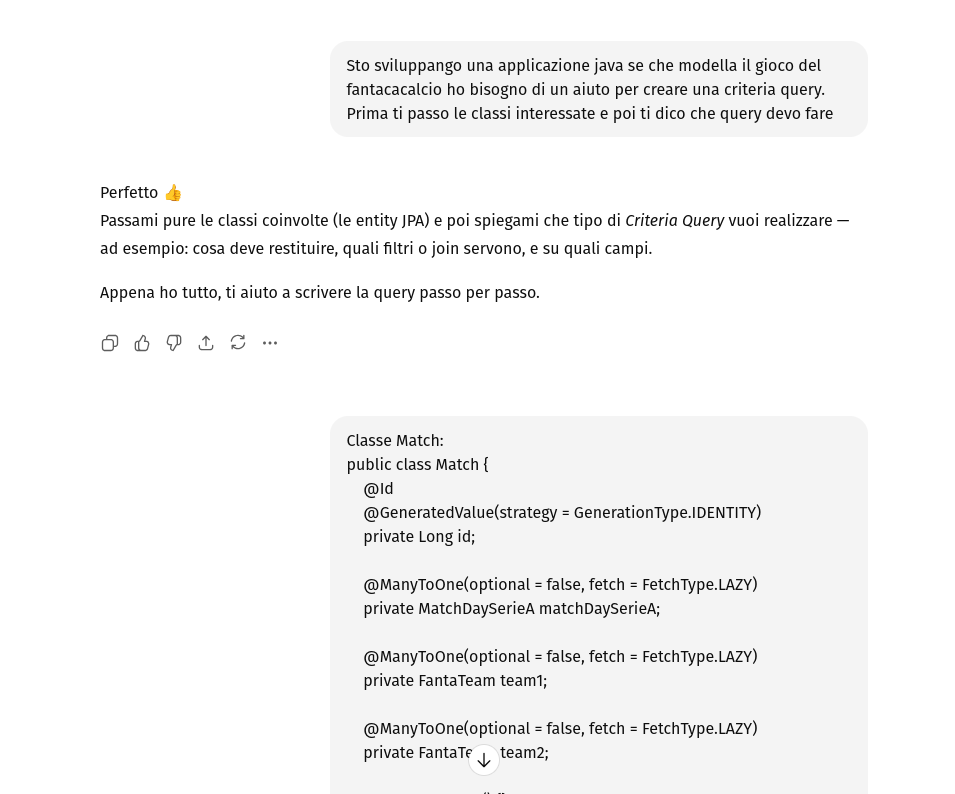
\includegraphics[width=\textwidth]{Resources/InterazioneLLMS/InterazioneParte1.png}        
    \caption{Interazione con LLMS parte 1.}
    \label{fig:interazione_con_LLMS_parte_1}
\end{figure}
\begin{figure}
    \centering
    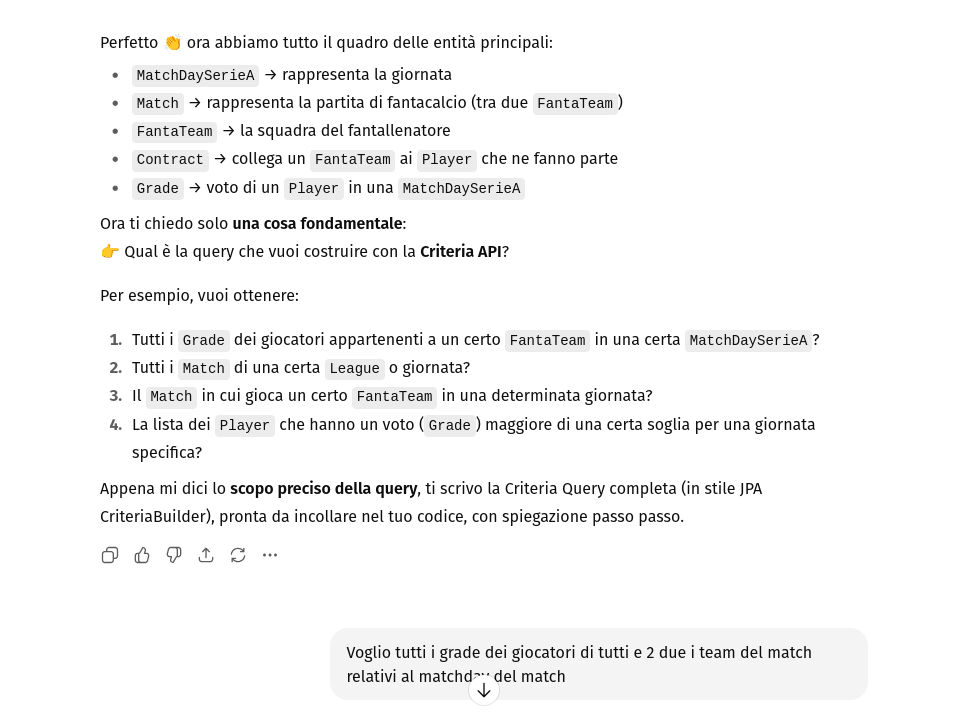
\includegraphics[width=\textwidth]{Resources/InterazioneLLMS/InterazioneParte2.png}        
    \caption{Interazione con LLMS parte 2.}
    \label{fig:interazione_con_LLMS_parte_2}
\end{figure}
\begin{figure}
    \centering
    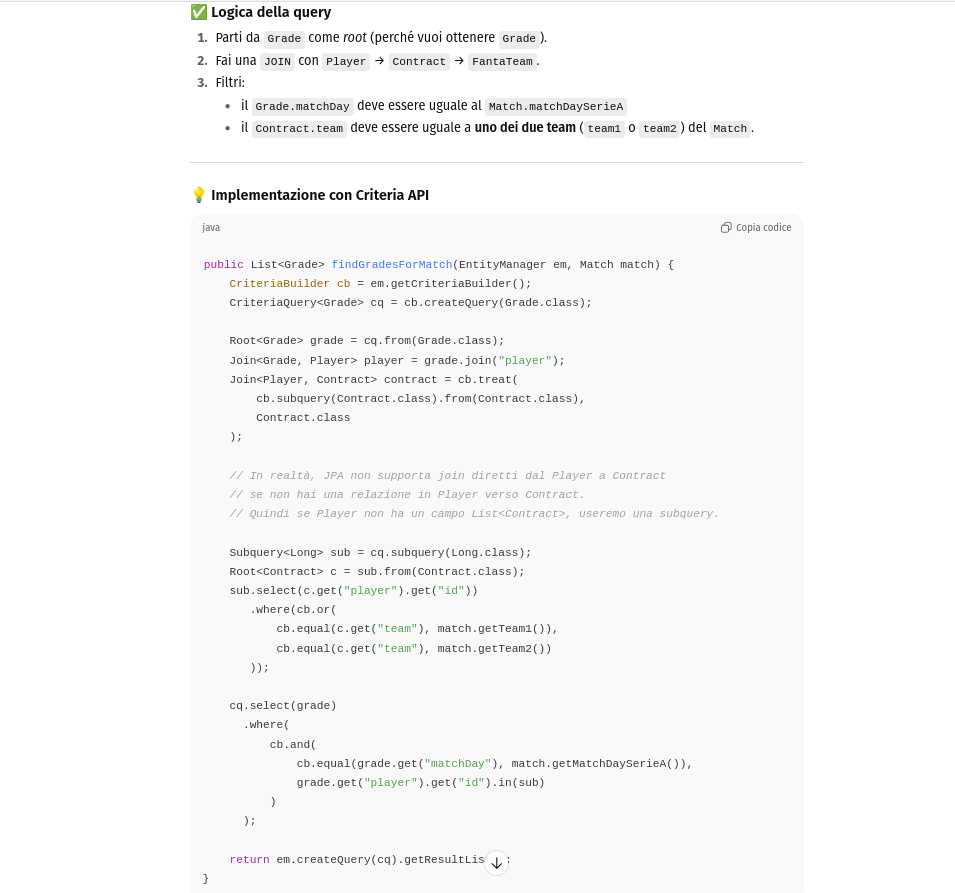
\includegraphics[width=\textwidth]{Resources/InterazioneLLMS/InterazioneParte3.png}        
    \caption{Interazione con LLMS parte 3.}
    \label{fig:interazione_con_LLMS_parte_3}
\end{figure}
\begin{figure}
    \centering
    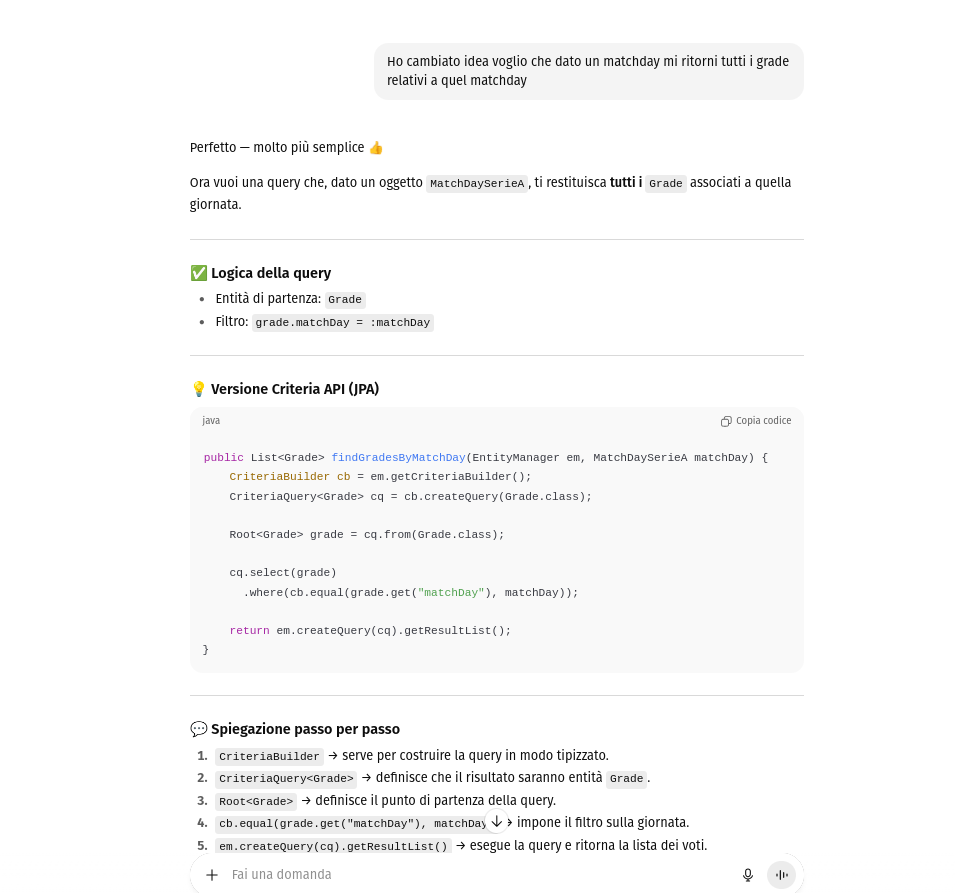
\includegraphics[width=\textwidth]{Resources/InterazioneLLMS/InterazioneParte4.png}        
    \caption{Interazione con LLMS parte 4.}
    \label{fig:interazione_con_LLMS_parte_4}
\end{figure}


\newpage
\begin{thebibliography}{9}
\bibitem{algLib}
\todo{Cosa ci mettiamo libro del vicario su jpa? poi? agag}

\end{thebibliography}

\end{document}